% Options for packages loaded elsewhere
% Options for packages loaded elsewhere
\PassOptionsToPackage{unicode}{hyperref}
\PassOptionsToPackage{hyphens}{url}
\PassOptionsToPackage{dvipsnames,svgnames,x11names}{xcolor}
%
\documentclass[
]{article}
\usepackage{xcolor}
\usepackage[margin=1in]{geometry}
\usepackage{amsmath,amssymb}
\setcounter{secnumdepth}{-\maxdimen} % remove section numbering
\usepackage{iftex}
\ifPDFTeX
  \usepackage[T1]{fontenc}
  \usepackage[utf8]{inputenc}
  \usepackage{textcomp} % provide euro and other symbols
\else % if luatex or xetex
  \usepackage{unicode-math} % this also loads fontspec
  \defaultfontfeatures{Scale=MatchLowercase}
  \defaultfontfeatures[\rmfamily]{Ligatures=TeX,Scale=1}
\fi
\usepackage{lmodern}
\ifPDFTeX\else
  % xetex/luatex font selection
\fi
% Use upquote if available, for straight quotes in verbatim environments
\IfFileExists{upquote.sty}{\usepackage{upquote}}{}
\IfFileExists{microtype.sty}{% use microtype if available
  \usepackage[]{microtype}
  \UseMicrotypeSet[protrusion]{basicmath} % disable protrusion for tt fonts
}{}
\makeatletter
\@ifundefined{KOMAClassName}{% if non-KOMA class
  \IfFileExists{parskip.sty}{%
    \usepackage{parskip}
  }{% else
    \setlength{\parindent}{0pt}
    \setlength{\parskip}{6pt plus 2pt minus 1pt}}
}{% if KOMA class
  \KOMAoptions{parskip=half}}
\makeatother
% Make \paragraph and \subparagraph free-standing
\makeatletter
\ifx\paragraph\undefined\else
  \let\oldparagraph\paragraph
  \renewcommand{\paragraph}{
    \@ifstar
      \xxxParagraphStar
      \xxxParagraphNoStar
  }
  \newcommand{\xxxParagraphStar}[1]{\oldparagraph*{#1}\mbox{}}
  \newcommand{\xxxParagraphNoStar}[1]{\oldparagraph{#1}\mbox{}}
\fi
\ifx\subparagraph\undefined\else
  \let\oldsubparagraph\subparagraph
  \renewcommand{\subparagraph}{
    \@ifstar
      \xxxSubParagraphStar
      \xxxSubParagraphNoStar
  }
  \newcommand{\xxxSubParagraphStar}[1]{\oldsubparagraph*{#1}\mbox{}}
  \newcommand{\xxxSubParagraphNoStar}[1]{\oldsubparagraph{#1}\mbox{}}
\fi
\makeatother


\usepackage{longtable,booktabs,array}
\newcounter{none} % for unnumbered tables
\usepackage{calc} % for calculating minipage widths
% Correct order of tables after \paragraph or \subparagraph
\usepackage{etoolbox}
\makeatletter
\patchcmd\longtable{\par}{\if@noskipsec\mbox{}\fi\par}{}{}
\makeatother
% Allow footnotes in longtable head/foot
\IfFileExists{footnotehyper.sty}{\usepackage{footnotehyper}}{\usepackage{footnote}}
\makesavenoteenv{longtable}
\usepackage{graphicx}
\makeatletter
\newsavebox\pandoc@box
\newcommand*\pandocbounded[1]{% scales image to fit in text height/width
  \sbox\pandoc@box{#1}%
  \Gscale@div\@tempa{\textheight}{\dimexpr\ht\pandoc@box+\dp\pandoc@box\relax}%
  \Gscale@div\@tempb{\linewidth}{\wd\pandoc@box}%
  \ifdim\@tempb\p@<\@tempa\p@\let\@tempa\@tempb\fi% select the smaller of both
  \ifdim\@tempa\p@<\p@\scalebox{\@tempa}{\usebox\pandoc@box}%
  \else\usebox{\pandoc@box}%
  \fi%
}
% Set default figure placement to htbp
\def\fps@figure{htbp}
\makeatother





\setlength{\emergencystretch}{3em} % prevent overfull lines

\providecommand{\tightlist}{%
  \setlength{\itemsep}{0pt}\setlength{\parskip}{0pt}}



 


\usepackage{lineno}
\linenumbers
\usepackage{float}
\usepackage[font=small,labelfont=bf]{caption}
\usepackage{lineno}
\linenumbers
\usepackage{float}
\usepackage[font=small,labelfont=bf]{caption}
\makeatletter
\@ifpackageloaded{caption}{}{\usepackage{caption}}
\AtBeginDocument{%
\ifdefined\contentsname
  \renewcommand*\contentsname{Table of contents}
\else
  \newcommand\contentsname{Table of contents}
\fi
\ifdefined\listfigurename
  \renewcommand*\listfigurename{List of Figures}
\else
  \newcommand\listfigurename{List of Figures}
\fi
\ifdefined\listtablename
  \renewcommand*\listtablename{List of Tables}
\else
  \newcommand\listtablename{List of Tables}
\fi
\ifdefined\figurename
  \renewcommand*\figurename{Figure}
\else
  \newcommand\figurename{Figure}
\fi
\ifdefined\tablename
  \renewcommand*\tablename{Table}
\else
  \newcommand\tablename{Table}
\fi
}
\@ifpackageloaded{float}{}{\usepackage{float}}
\floatstyle{ruled}
\@ifundefined{c@chapter}{\newfloat{codelisting}{h}{lop}}{\newfloat{codelisting}{h}{lop}[chapter]}
\floatname{codelisting}{Listing}
\newcommand*\listoflistings{\listof{codelisting}{List of Listings}}
\makeatother
\makeatletter
\makeatother
\makeatletter
\@ifpackageloaded{caption}{}{\usepackage{caption}}
\@ifpackageloaded{subcaption}{}{\usepackage{subcaption}}
\makeatother
\usepackage{bookmark}
\IfFileExists{xurl.sty}{\usepackage{xurl}}{} % add URL line breaks if available
\urlstyle{same}
\hypersetup{
  pdftitle={The metabolic cost of the febrile host across priority Candida species},
  pdfauthor={Ilgaz Cakin},
  colorlinks=true,
  linkcolor={blue},
  filecolor={Maroon},
  citecolor={Blue},
  urlcolor={Blue},
  pdfcreator={LaTeX via pandoc}}


\title{The metabolic cost of the febrile host across priority Candida
species}
\author{Ilgaz Cakin}
\date{}
\begin{document}
\maketitle


\emph{Results}

We tested whether warming imposes a metabolic cost on pathogenic
\emph{Candida} by raising respiration relative to growth. Across all
taxa, growth peaked below fever temperature while respiration continued
to rise, so carbon-use efficiency declined at host temperatures, and the
penalty was substantially smaller in the most thermotolerant \emph{C.
auris} clades.

Dissolved-oxygen respirometry was used to fit thermal performance curves
for four Candida \emph{auris} clades (I-IV; three isolates each) and C.
\emph{parapsilosis} (three isolates), across 22-44 °C (12 temperatures).
Growth was modelled with a Sharpe-Schoolfield function and per-cell
respiration with a Boltzmann-Arrhenius function, both fitted
hierarchically (isolates nested within clades) in a Bayesian framework.
Unless stated, values are posterior medians with 95\% credible intervals
(CrI).

\subsection{\texorpdfstring{\textbf{Methods
(summary)}}{Methods (summary)}}\label{methods-summary}

O\textsubscript{2} concentration was recorded continuously with PreSens
SensorDish readers across the temperature series (22-44 °C, 12
temperatures; three isolates × five replicates per temperature).
Specific growth rate and per-cell respiration rate were recovered
simultaneously from each O\textsubscript{2} time series using the
mechanistic oxygen-dynamics model of Cakin \emph{et al.} (2026), which
couples exponential population growth with biomass-proportional oxygen
consumption, O\textsubscript{2}(t) = O\textsubscript{2,0} + (K/r)(1 −
e\textsuperscript{rt}), where r is the specific growth rate and K the
volumetric O\textsubscript{2} consumption rate at the window start.
Per-cell respiration, carbon-use efficiency and derived quantities were
computed as in that study.

Growth and respiratory carbon flux were expressed on a matched per-cell
basis, so carbon-use efficiency could be computed as CUE = G/(G + R).
Because the assumed per-cell carbon quota is temperature-independent,
the activation energy of growth is directly comparable with that of
respiration.

\section{\texorpdfstring{\textbf{Growth and respiration decouple,
placing the carbon-economy optimum below body
temperature}}{Growth and respiration decouple, placing the carbon-economy optimum below body temperature}}\label{growth-and-respiration-decouple-placing-the-carbon-economy-optimum-below-body-temperature}

Growth rate rose with temperature to a clade-level optimum near 33-36 °C
and then declined, following the expected unimodal thermal performance
curve (Fig. 1a). Per-cell respiration showed no such turnover: it
increased monotonically across the entire measured range, and
leave-one-out cross-validation favoured the monotonic Arrhenius model
over a unimodal Sharpe-Schoolfield alternative (Fig. 1b). Growth and
respiration are therefore governed by different thermal sensitivities.

This difference is quantified by the activation energies (Fig. 1c). In
every taxon, the activation energy of growth exceeded that of
respiration: E\textsubscript{G} ranged 0.83-1.14 eV and
E\textsubscript{R} 0.30-0.52 eV, with the growth-respiration difference
credibly greater than zero in all five taxa (0.39-0.73 eV; 95\% CrI
excluding zero throughout). Growth is thus substantially more
temperature-sensitive than respiration. The respiration activation
energies additionally carry a temperature-structured uncertainty from
the inoculum back-projection (Robustness, below); this shifts their
absolute values but not the growth-minus-respiration ordering in any
taxon, which is the comparison that matters here.

Because respiration continues to rise while growth saturates and falls,
carbon-use efficiency (CUE = G/(G+R)) is itself a unimodal function of
temperature that peaks early and then collapses (Fig. 1d). The
temperature of this economic optimum, T\textsubscript{opt}(CUE) lay
below human body temperature in every taxon: 31.3-34.1 °C, with
posterior probability P(T\textsubscript{opt}(CUE) \textless{} 37 °C) ≥
0.999 for all five (Fig. 1e). The economic optimum sat 1.6-3.9 °C below
the growth optimum and 2.9-5.7 °C below 37 °C. The mammalian host
temperature therefore lies beyond the point at which warming still
improves the carbon economy of any species tested.

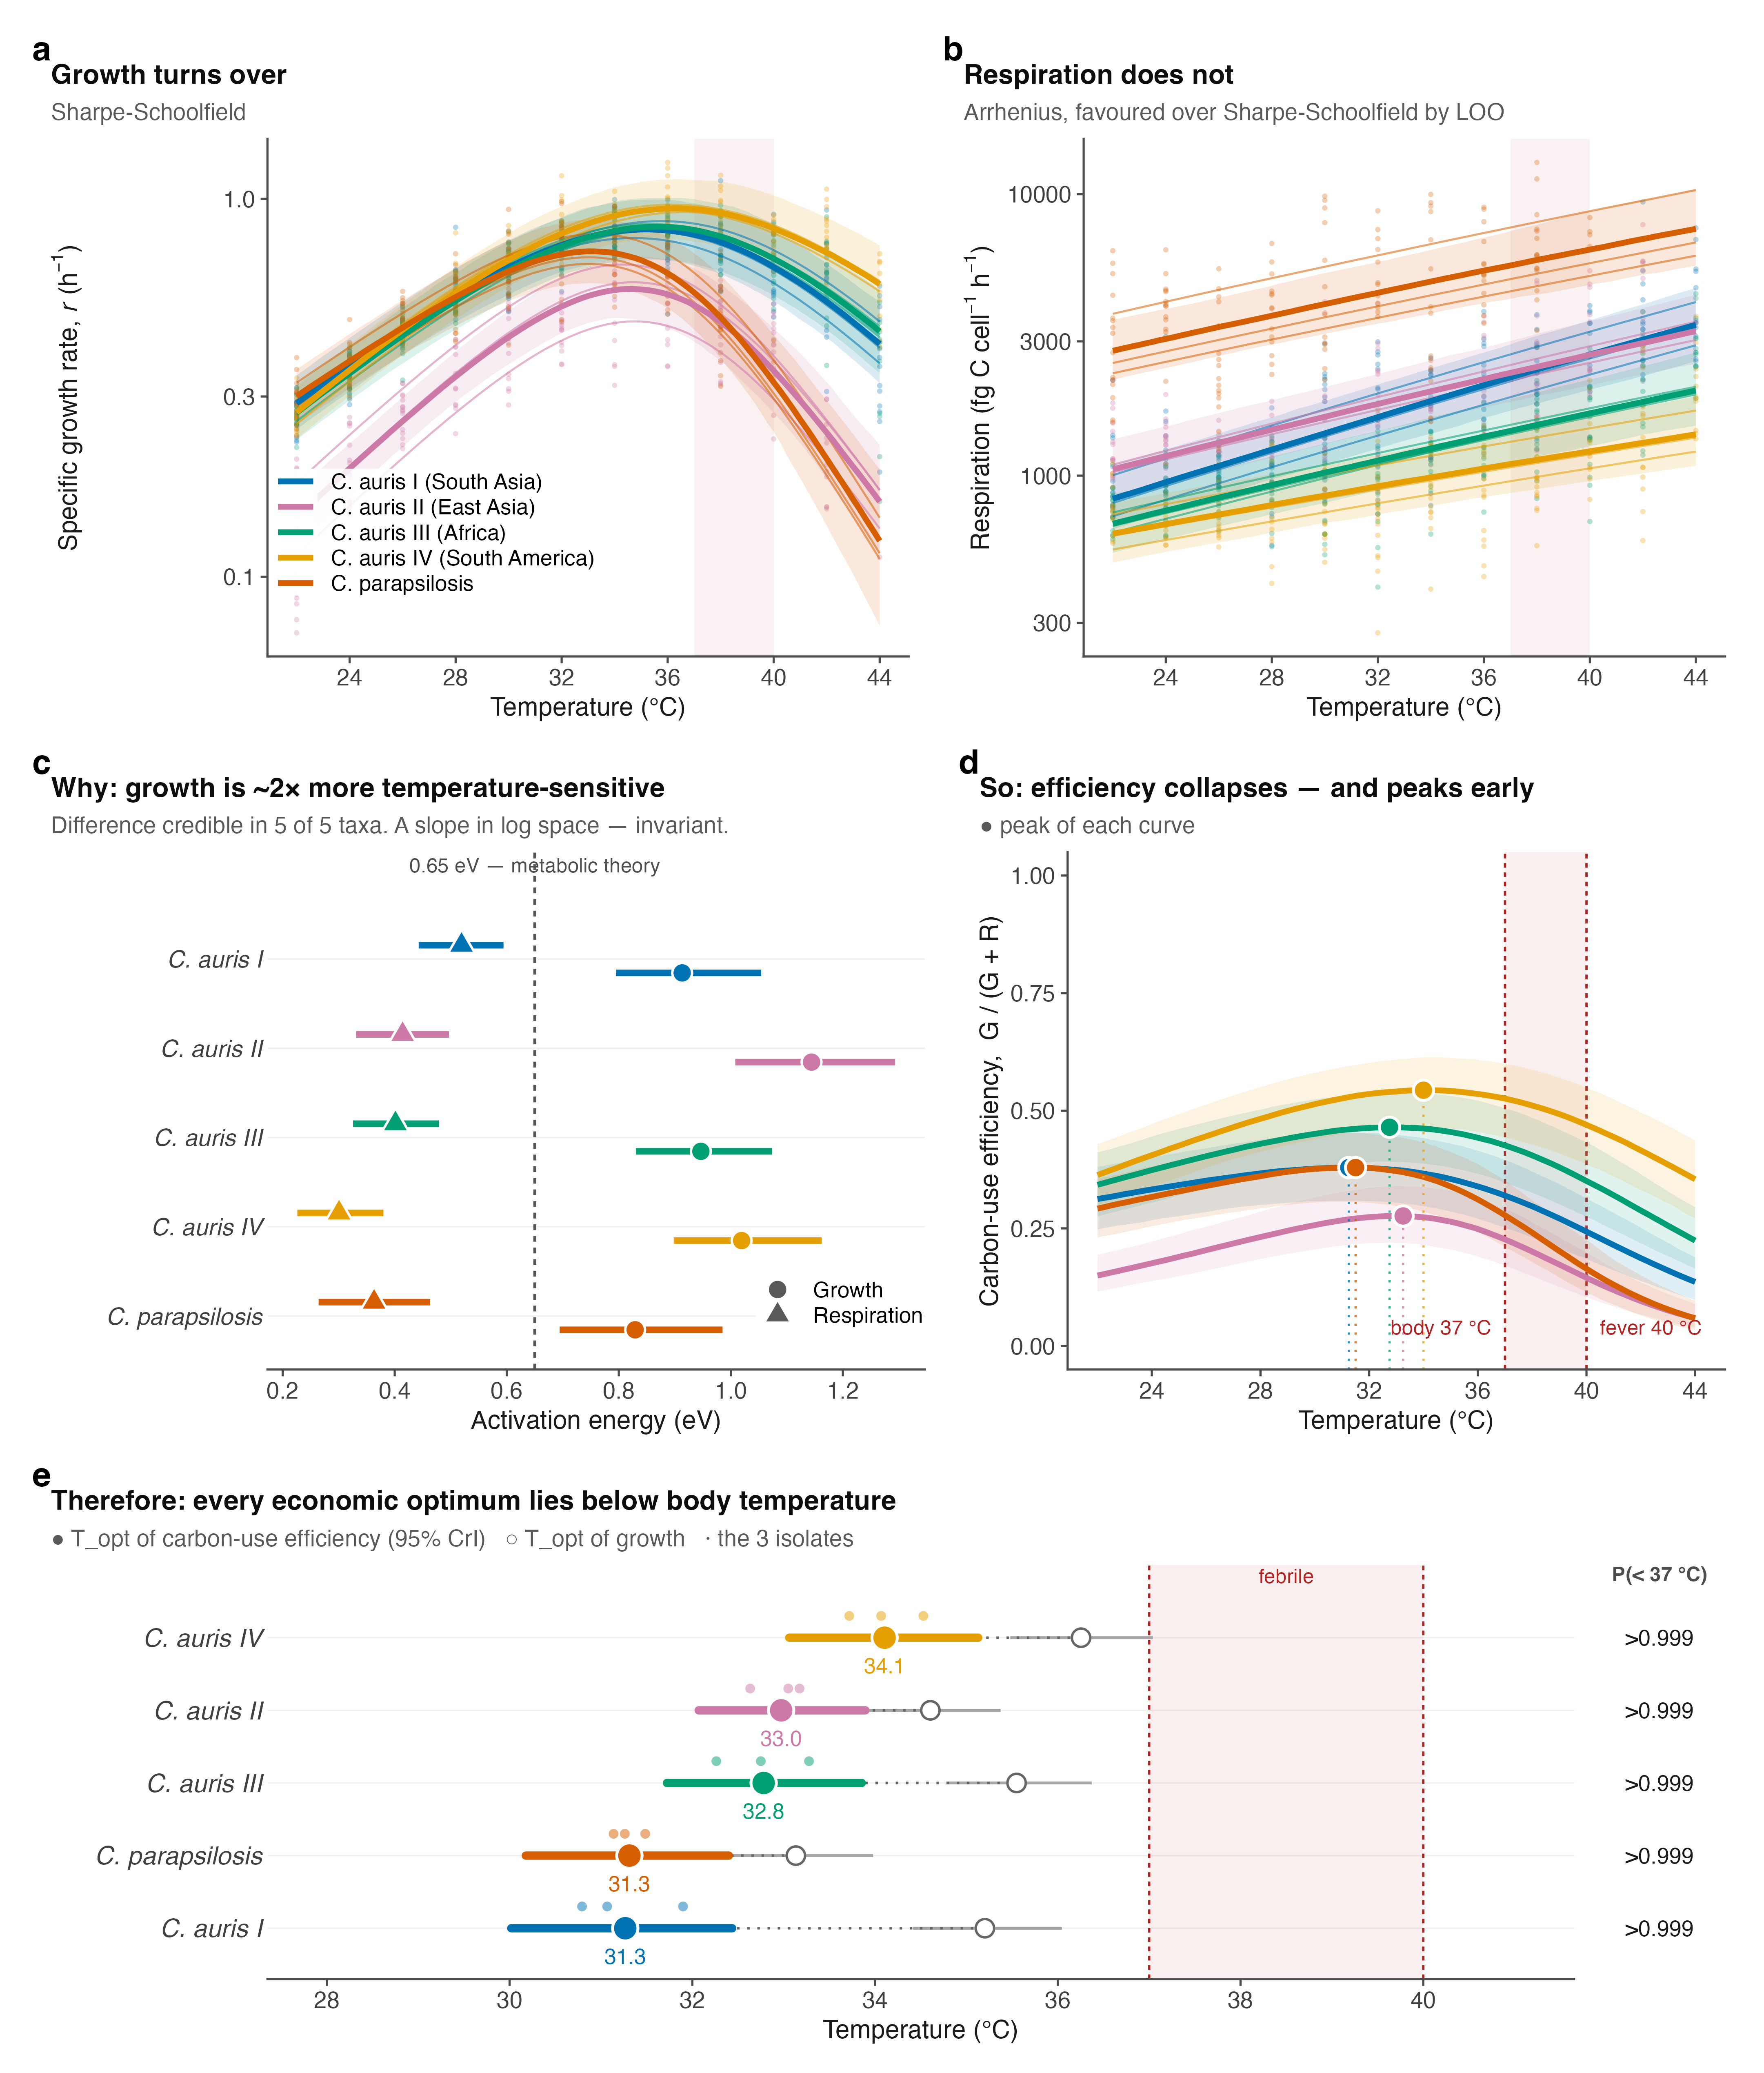
\includegraphics[width=6.39583in,height=7.51459in]{media/media/image1.png}

\textbf{Figure 1. Growth and respiration decouple with temperature,
placing every carbon-economy optimum below body temperature.}
(\textbf{a}) Specific growth rate \emph{r} (h⁻¹) and (\textbf{b})
per-cell respiration carbon flux (fg C cell⁻¹ h⁻¹) versus temperature
(points, isolate-level observations; thin lines, per-isolate fits; bold
lines, clade-level posterior medians; bands, 95\% CrI). Growth turns
over; respiration does not (Arrhenius favoured over Sharpe-Schoolfield
by leave-one-out cross-validation). (\textbf{c}) Activation energies of
growth (circles) and respiration (triangles); dashed line, the 0.65 eV
metabolic-theory value. Growth is credibly more temperature-sensitive
than respiration in all five taxa. (\textbf{d}) Carbon-use efficiency,
CUE = G/(G+R), collapses with warming and peaks early; filled points
mark each curve's peak. (\textbf{e}) Thermal optimum of CUE (filled
points, 95\% CrI; open points, growth optimum; small points, isolates),
with the posterior probability that it lies below 37 °C. Shaded band, 37
to 40 °C (body to fever).

\textbf{A febrile host imposes a quantifiable, taxon-specific carbon
tax}

Because the economic optimum lies below 37 °C, every taxon operates at a
carbon penalty in the host. We express this as the relative respiratory
cost, i.e.~respiration per unit growth relative to each taxon's own
cheapest temperature (Fig. 2a). At 40 °C (fever), this cost reached
1.34× for C. \emph{auris} Clade IV but 3.13× for C. \emph{parapsilosis}.

The three-degree step from body temperature (37 °C) to fever (40 °C)
captures the clinical penalty most directly (Fig. 2c). Over this
interval C. \emph{parapsilosis} retained only 58\% of its 37 °C growth
rate (0.58, 95\% CrI 0.50-0.67) while its respiratory cost per unit
growth rose 1.96× (1.71-2.31). The C. \emph{auris} clades were far less
affected: Clade IV retained 89\% of growth (0.89, 0.85-0.93) at a cost
increase of only 1.25× (1.19-1.31), with Clades I-III intermediate
(growth retained 0.67-0.84; cost 1.37×-1.73×). Fever thus suppresses
growth without suppressing respiration, and it does so most severely in
C. \emph{parapsilosis}. Absolute per-cell costs at 40 °C carry the
temperature-equilibration uncertainty quantified below; the direction
and the among-taxon ranking are unaffected.

\textbf{Clade-level differences within} C. \emph{auris}\textbf{.}
Pairwise comparison of the fever cost resolved 8 of 10 taxon contrasts
(95\% CrI excluding a ratio of 1; Fig. 2d). All four C. \emph{auris}
clades credibly paid less at fever than C. \emph{parapsilosis} (cost
ratios 0.43-0.72); this contrast is the robust result and holds under
every treatment of the inoculum back-projection (Robustness). Within C.
\emph{auris}, Clade IV had the lowest fever cost under the
back-projection used throughout, but the fine ranking among the four
clades is the one result sensitive to how N0 is handled: it does not
survive removal of the back-projection term (Robustness; Supplementary
Fig. 6), so we report Clade IV as the cheapest under the analysis as
specified rather than as an unconditional ordering. Only two contrasts,
Clade I versus Clade II (0.85, 0.68-1.04) and Clade I versus Clade III
(1.18, 0.98-1.42), could not be separated at three isolates per clade.

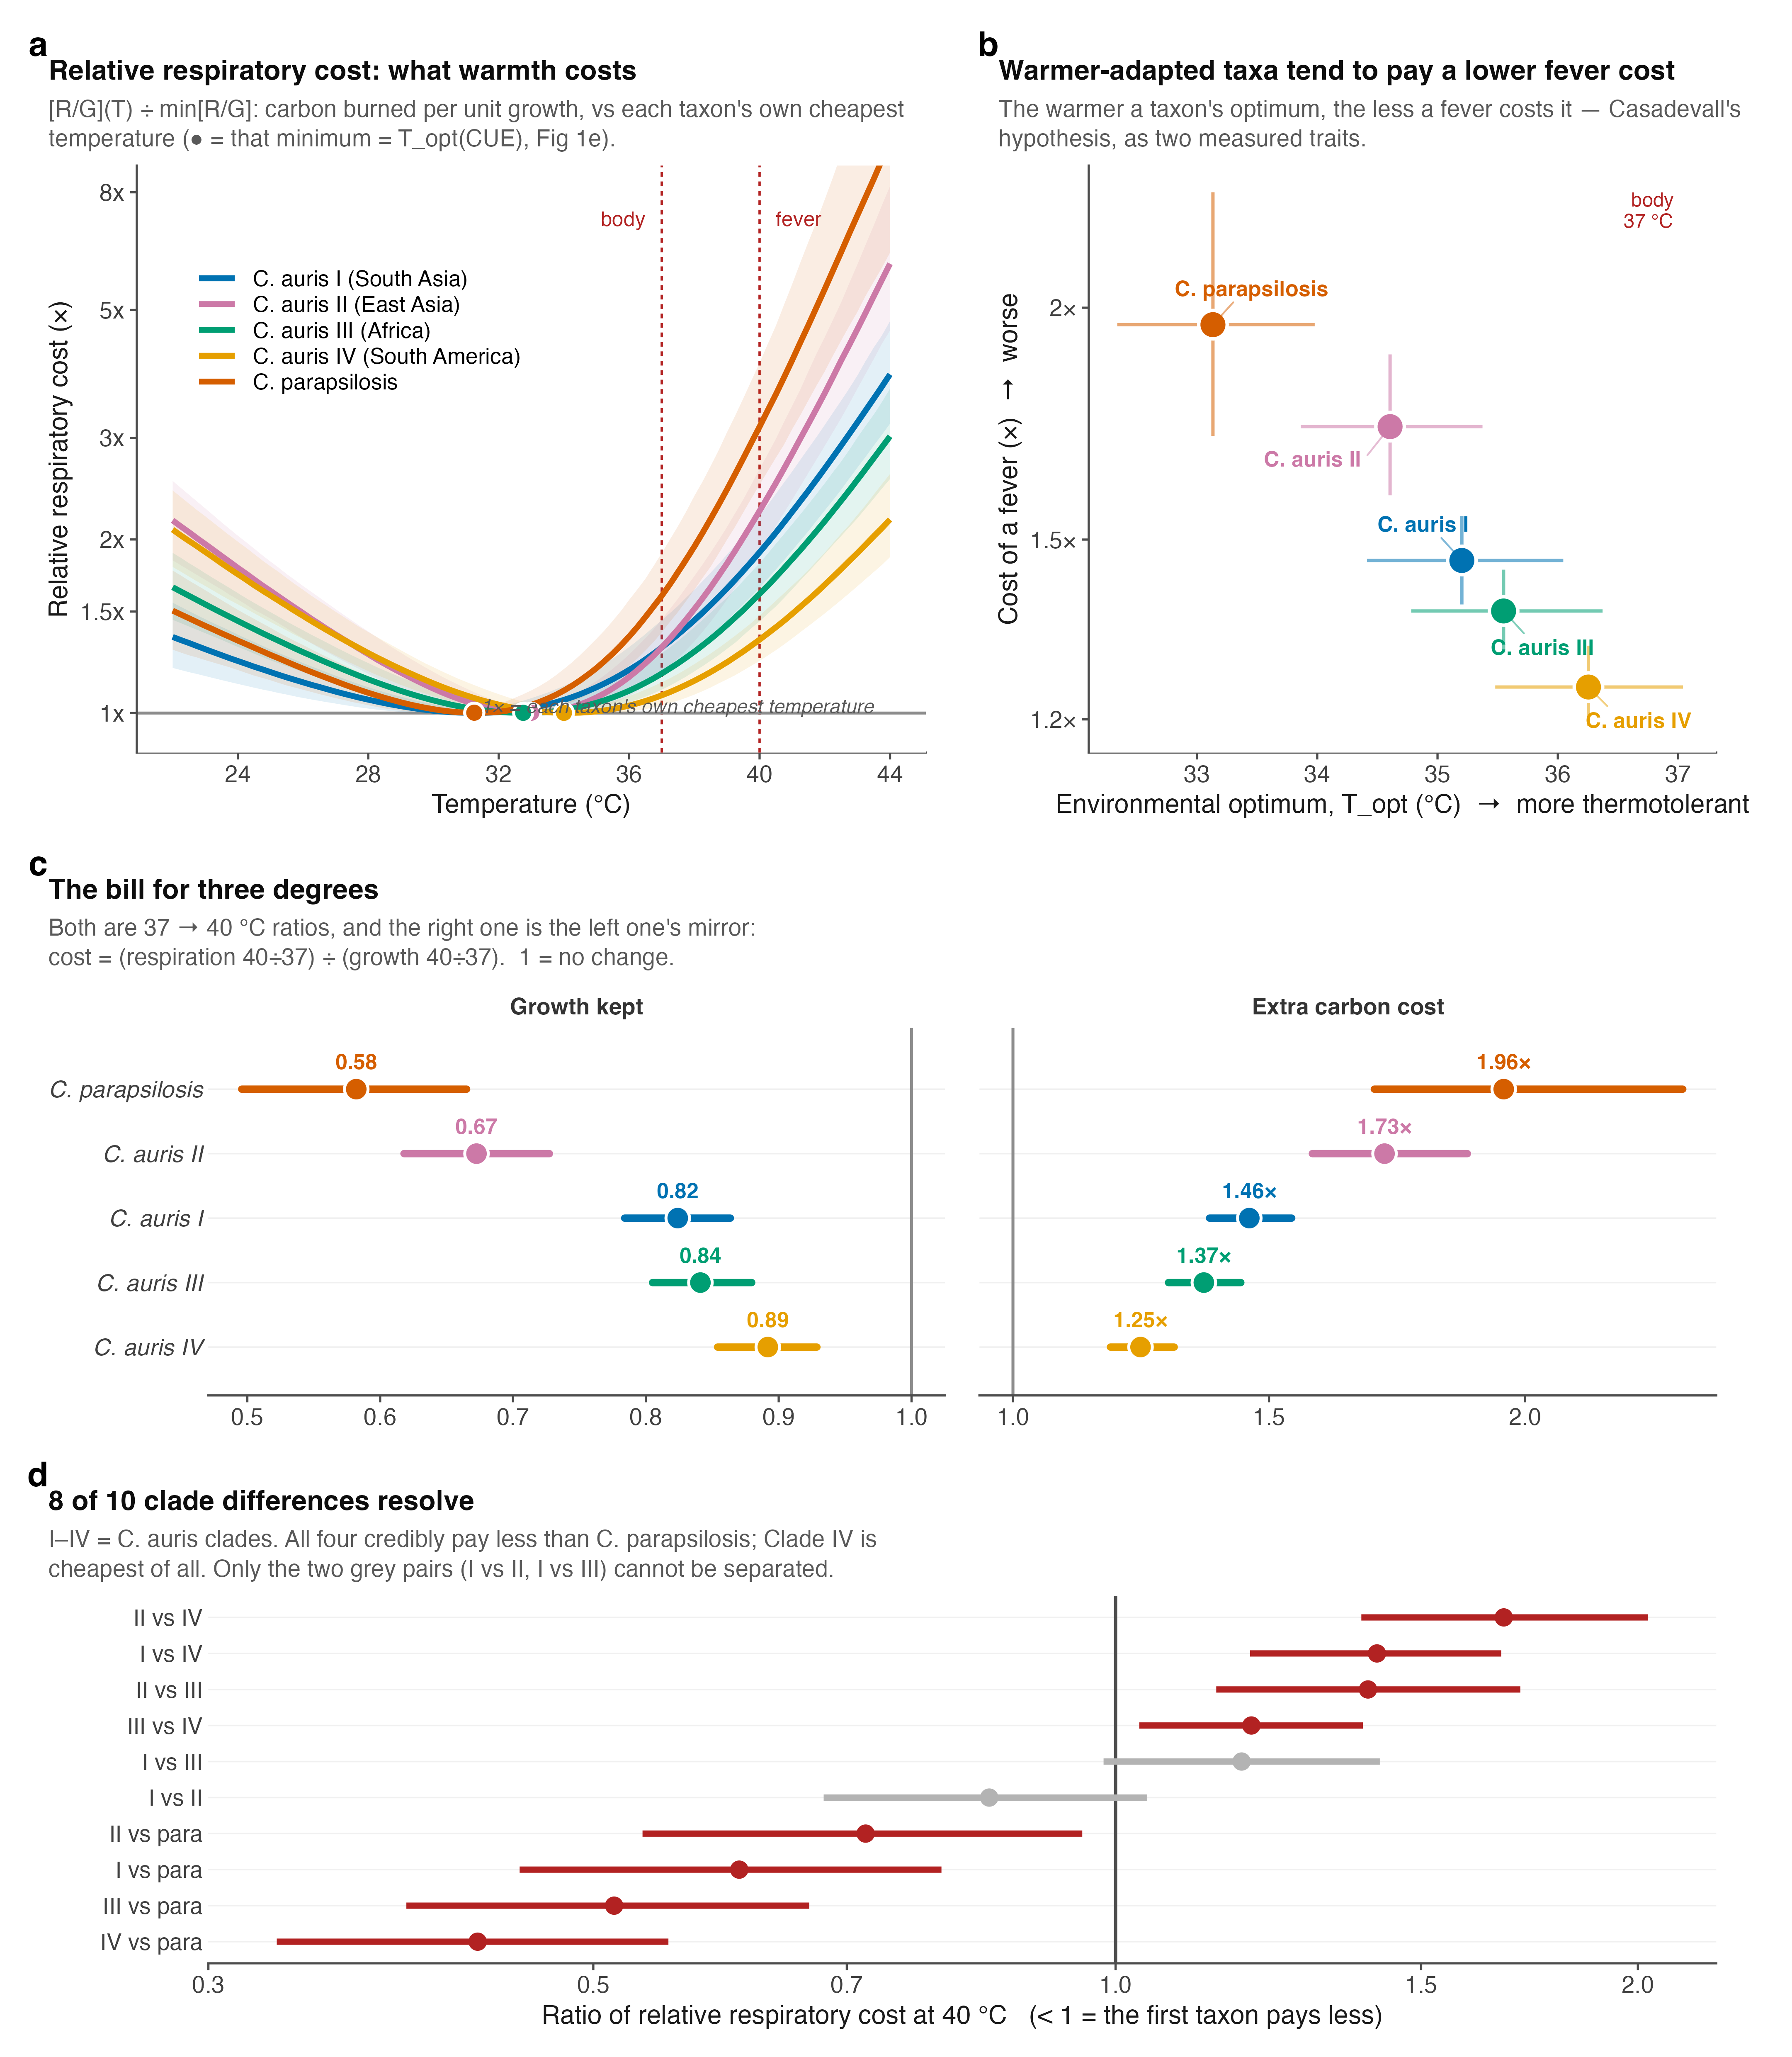
\includegraphics[width=6.39583in,height=7.33997in]{media/media/image2.png}

\textbf{Figure 2.} A febrile host imposes a quantifiable, taxon-specific
carbon cost. (a) Relative respiratory cost (respiration per unit growth,
each taxon normalised to its own cheapest temperature) versus
temperature; the minimum marks the CUE optimum, Topt(CUE). (b)
Environmental growth optimum versus the cost of a fever across the five
taxa; warmer-adapted taxa pay less. (c) The 37 to 40 °C step: growth
retained (left) and the rise in respiratory cost per unit growth
(right). (d) Pairwise contrasts of the 40 °C fever cost among clades and
against \emph{C. parapsilosis} (ratio \textless{} 1 means the first
taxon pays less). Points and bars are posterior medians with 95\%
credible intervals.

As an exploratory observation resting on only five taxa, and one partly
geometrically coupled to the growth curve, the environmental growth
optimum was negatively associated with the cost of a fever: the more
thermotolerant a taxon, the less a fever cost it (Fig. 2b). Computed as
a posterior over Spearman's ρ (propagating parameter uncertainty rather
than treating the five taxon medians as fixed), the correlation was ρ =
−0.90 (95\% CrI −1.00 to −0.30; P(ρ \textless{} 0) = 0.996), with
\emph{C. parapsilosis} at the cool-optimum, expensive-fever extreme and
\emph{C. auris} Clade IV at the warm-optimum, cheap-fever extreme. The
respiration activation energy is an independent parameter that could
have broken the relationship and did not; with only five points,
however, we report the association as suggestive, to be tested directly
with additional species. It is consistent with environmental thermal
selection contributing to tolerance of the mammalian host.

Temperature-equilibration uncertainty in the inoculum back-projection
affected the absolute per-cell values most at the temperature extremes
(≥40 °C) but changed neither the direction nor the significance of these
results, and preserved the C. \emph{auris}-versus-\emph{C. parapsilosis}
ordering. The finer ranking among the C. \emph{auris} clades is more
sensitive to the back-projection and is treated as conditional
throughout (Robustness and limitations).

\textbf{Clade differences are captured by an effective growth-capacity
axis despite near-identical sequences}

Having established reproducible differences in fever cost among the
\emph{C. auris} clades, we asked whether their near-identical enzyme
sequences could account for them. We compared the measured growth curves
with a sequence-grounded, enzyme- and temperature-constrained
genome-scale metabolic model (etc-GEM), in which fixed genome-derived
inputs feed a model that maximises growth at each temperature under a
shared enzyme budget, and three parameters are calibrated to each
clade's growth curve (Fig. 3).

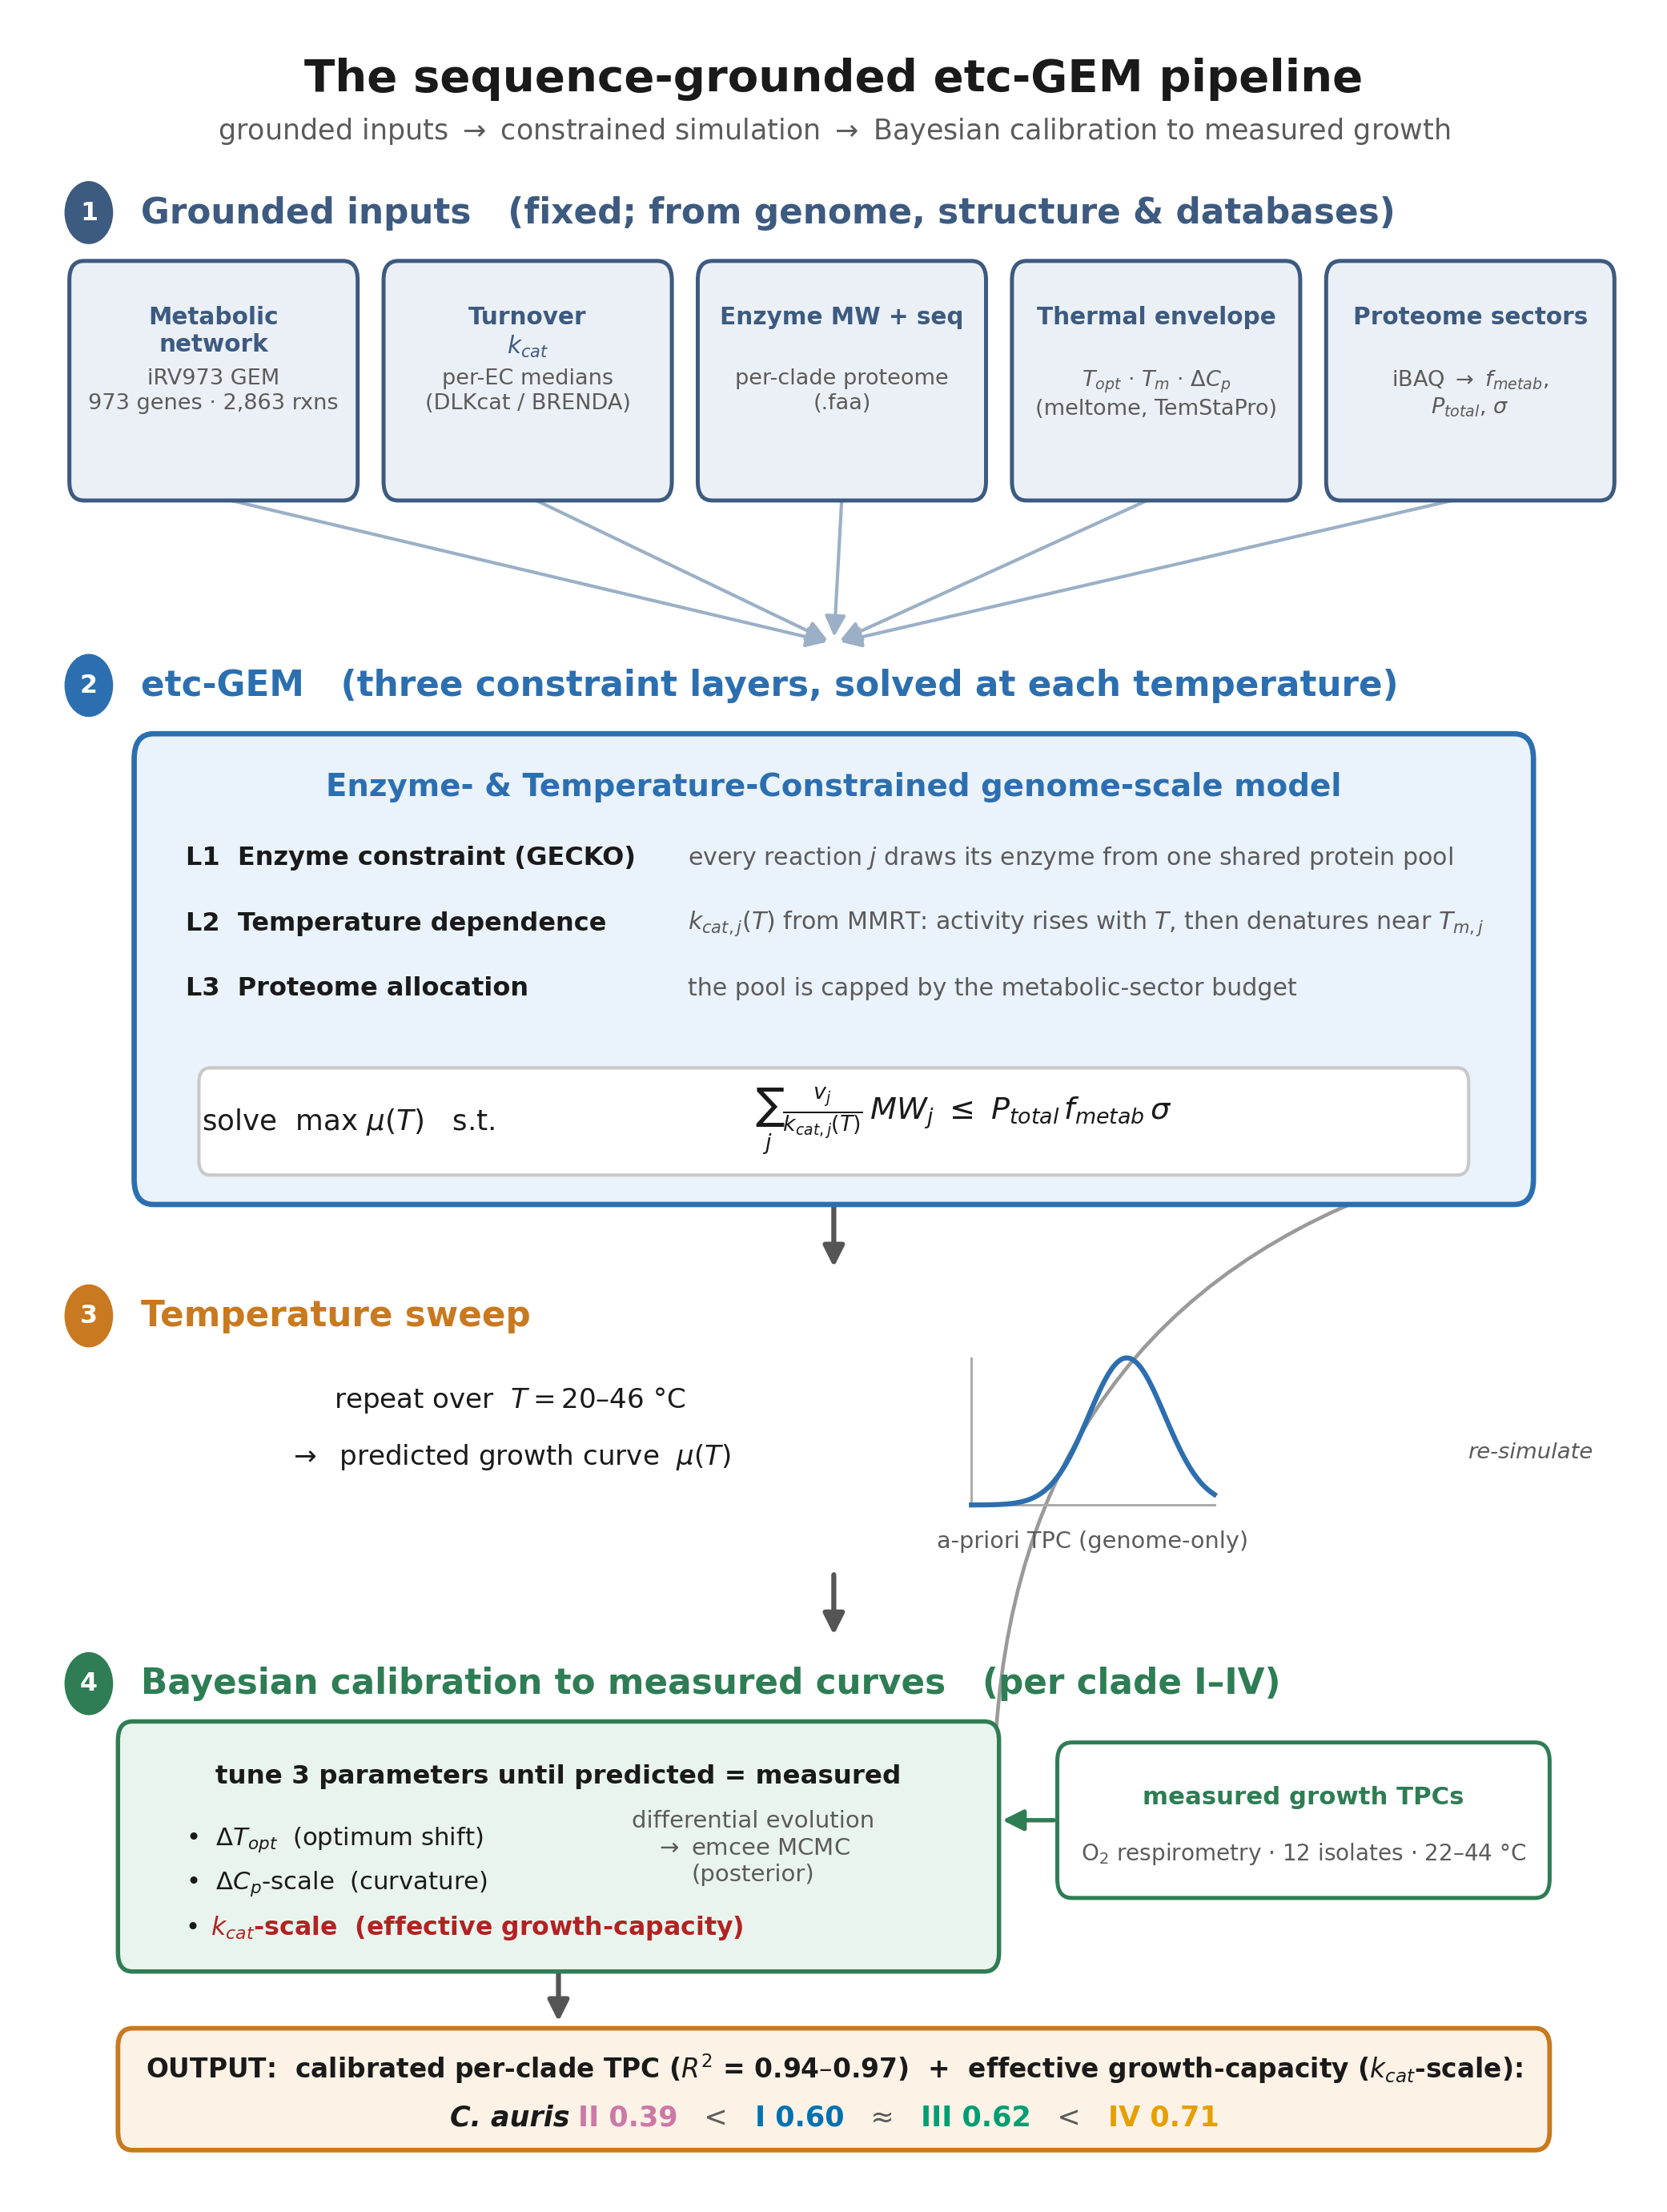
\includegraphics[width=5.5993in,height=7.45229in]{media/media/image3.png}

\textbf{Figure 3.} The sequence-grounded etc-GEM pipeline. Fixed,
genome-derived inputs (the iRV973 metabolic network; per-reaction
turnover kcat from EC/DLKcat; enzyme molecular weights and per-clade
sequences; per-enzyme thermal parameters Topt, Tm and ΔCp; and
proteome-sector fractions) feed an enzyme- and temperature-constrained
genome-scale model that, at each temperature, maximises growth subject
to a shared enzyme budget. Three parameters (ΔTopt, ΔCp-scale, and
effective-capacity kcat-scale) are then calibrated by differential
evolution and MCMC to each clade's measured growth curve. Within the
calibrated model, the effective growth-capacity axis is the only
parameter that clearly separates the clades, despite their
\textgreater99\% reference-proteome identity; the per-clade values are
given in Figure 4.

The four clades are near-identical at the enzyme level: median
whole-proteome amino-acid identity was 99.4-100\% across clades I-IV
(reciprocal best-hit alignment of the four reference proteomes).
Consequently the genome-derived model predicts a nearly identical
thermal curve for all four clades, whereas their measured peak growth
differs roughly two-fold (Fig. 4b). Broad differences in enzyme coding
sequence are therefore unlikely to explain the observed clade
differences.

The difference is captured instead by an effective growth-capacity axis
(kcat-scale), an effective flux-generating capacity per unit modelled
metabolic proteome that lumps enzyme abundance, active fraction,
substrate saturation, maintenance and respiratory coupling (Fig. 4c). It
is a single proteome-wide capacity scaling, not a change in the
individual database-derived kcat values, which are shared across the
near-identical clades. Its posterior ordered with thermotolerance (Clade
II lowest at 0.39, Clades I and III intermediate at 0.60 and 0.62, Clade
IV highest at 0.71), and of the three calibration parameters it was the
only one that separated the clades (5 of 6 pairwise contrasts with
non-overlapping 95\% CrI, versus 1 of 6 for the optimum shift and 0 of 6
for curvature; Supplementary Fig. 1b).

The effective-capacity axis covaries with measured respiratory
economics. The growth-fitted scalar covaried across the twelve isolates
with outcomes not used to fit the model and that incorporate measured
respiration: it was negatively associated with the cost of a fever (r =
−0.86, 95\% CI −0.96 to −0.76), so the higher a clade's capacity the
cheaper its fever (Fig. 4d), and with per-cell respiration at the growth
optimum (r = −0.64), so that higher-capacity clades sustain growth while
respiring less carbon (Fig. 4e). This second association is itself
sensitive to the inoculum back-projection: removing the back-projection
term weakens it to r ≈ −0.2 (not significant), so we treat the
capacity-versus-respiration relationship (Fig. 4e) as exploratory
(Robustness). The capacity-versus-fever-cost relationship (Fig. 4d) is
the more stable of the two but, being derived from the same respiration
measurements, is read in the same cross-phenotype rather than
confirmatory sense (below). Capacity behaved as a reproducible
clade-level trait, with 90\% of its variance falling between clades
(ICC₁ = 0.90; ANOVA F₃,₈ = 27.7, P = 1.4×10⁻⁴; Supplementary Fig. 1a).

These are cross-phenotype associations, not independent mechanistic
validation. First, the fever tax is itself derived from measured growth
and respiration through carbon-use efficiency, so it is not a fully
independent target. Second, a flux-variability analysis showed that
oxygen consumption at fixed optimal growth is not uniquely determined by
the growth-calibrated model, so the model's respiration is an
objective-selected flux solution rather than a unique prediction. Third,
growth-only fits of alternative capacity, maintenance and uptake
constraints each reproduced the clade growth ranking but none recovered
the observed ranking in respiratory cost, with Clade II combining the
lowest growth with the highest respiratory cost. We therefore read the
fitted parameter as an effective growth-capacity axis that does not by
itself distinguish reduced enzyme deployment from a coupling or
maintenance component. The capacity-versus-peak-growth relationship, by
contrast, is a self-consistency check rather than independent evidence,
because capacity is itself the fitted height term (Supplementary Fig.
2).

The near-identity of the reference proteomes makes broad coding-sequence
divergence an unlikely explanation for the capacity differences. A
direct transcriptional test likewise did not support a coordinated
relative down-allocation of metabolic transcripts: in the only public
clade-resolved RNA-seq at a controlled condition (Clade I versus Clade
II, 37 °C; GEO GSE165762), the model's 928 central-metabolic enzyme
genes were not coordinately lower in the low-capacity clade (median log₂
fold-change -0.005 versus +0.031 for the genome background; Wilcoxon P =
0.93; Supplementary Fig. 1d). Because that analysis is compositional
(standard library-size-normalised RNA-seq, a single Clade II isolate,
one 37 °C snapshot), it rules out a relative down-allocation of
metabolic transcripts, not lower absolute output. The causal layer is
therefore non-coding, regulatory, post-transcriptional,
post-translational, or bioenergetic, and remains undetermined among
these; distinguishing them will require a model-identifiability analysis
(profiling capacity against maintenance, uptake and respiratory
coupling) together with absolute, spike-in-calibrated proteomics, which
partitions but does not fully close these branches.

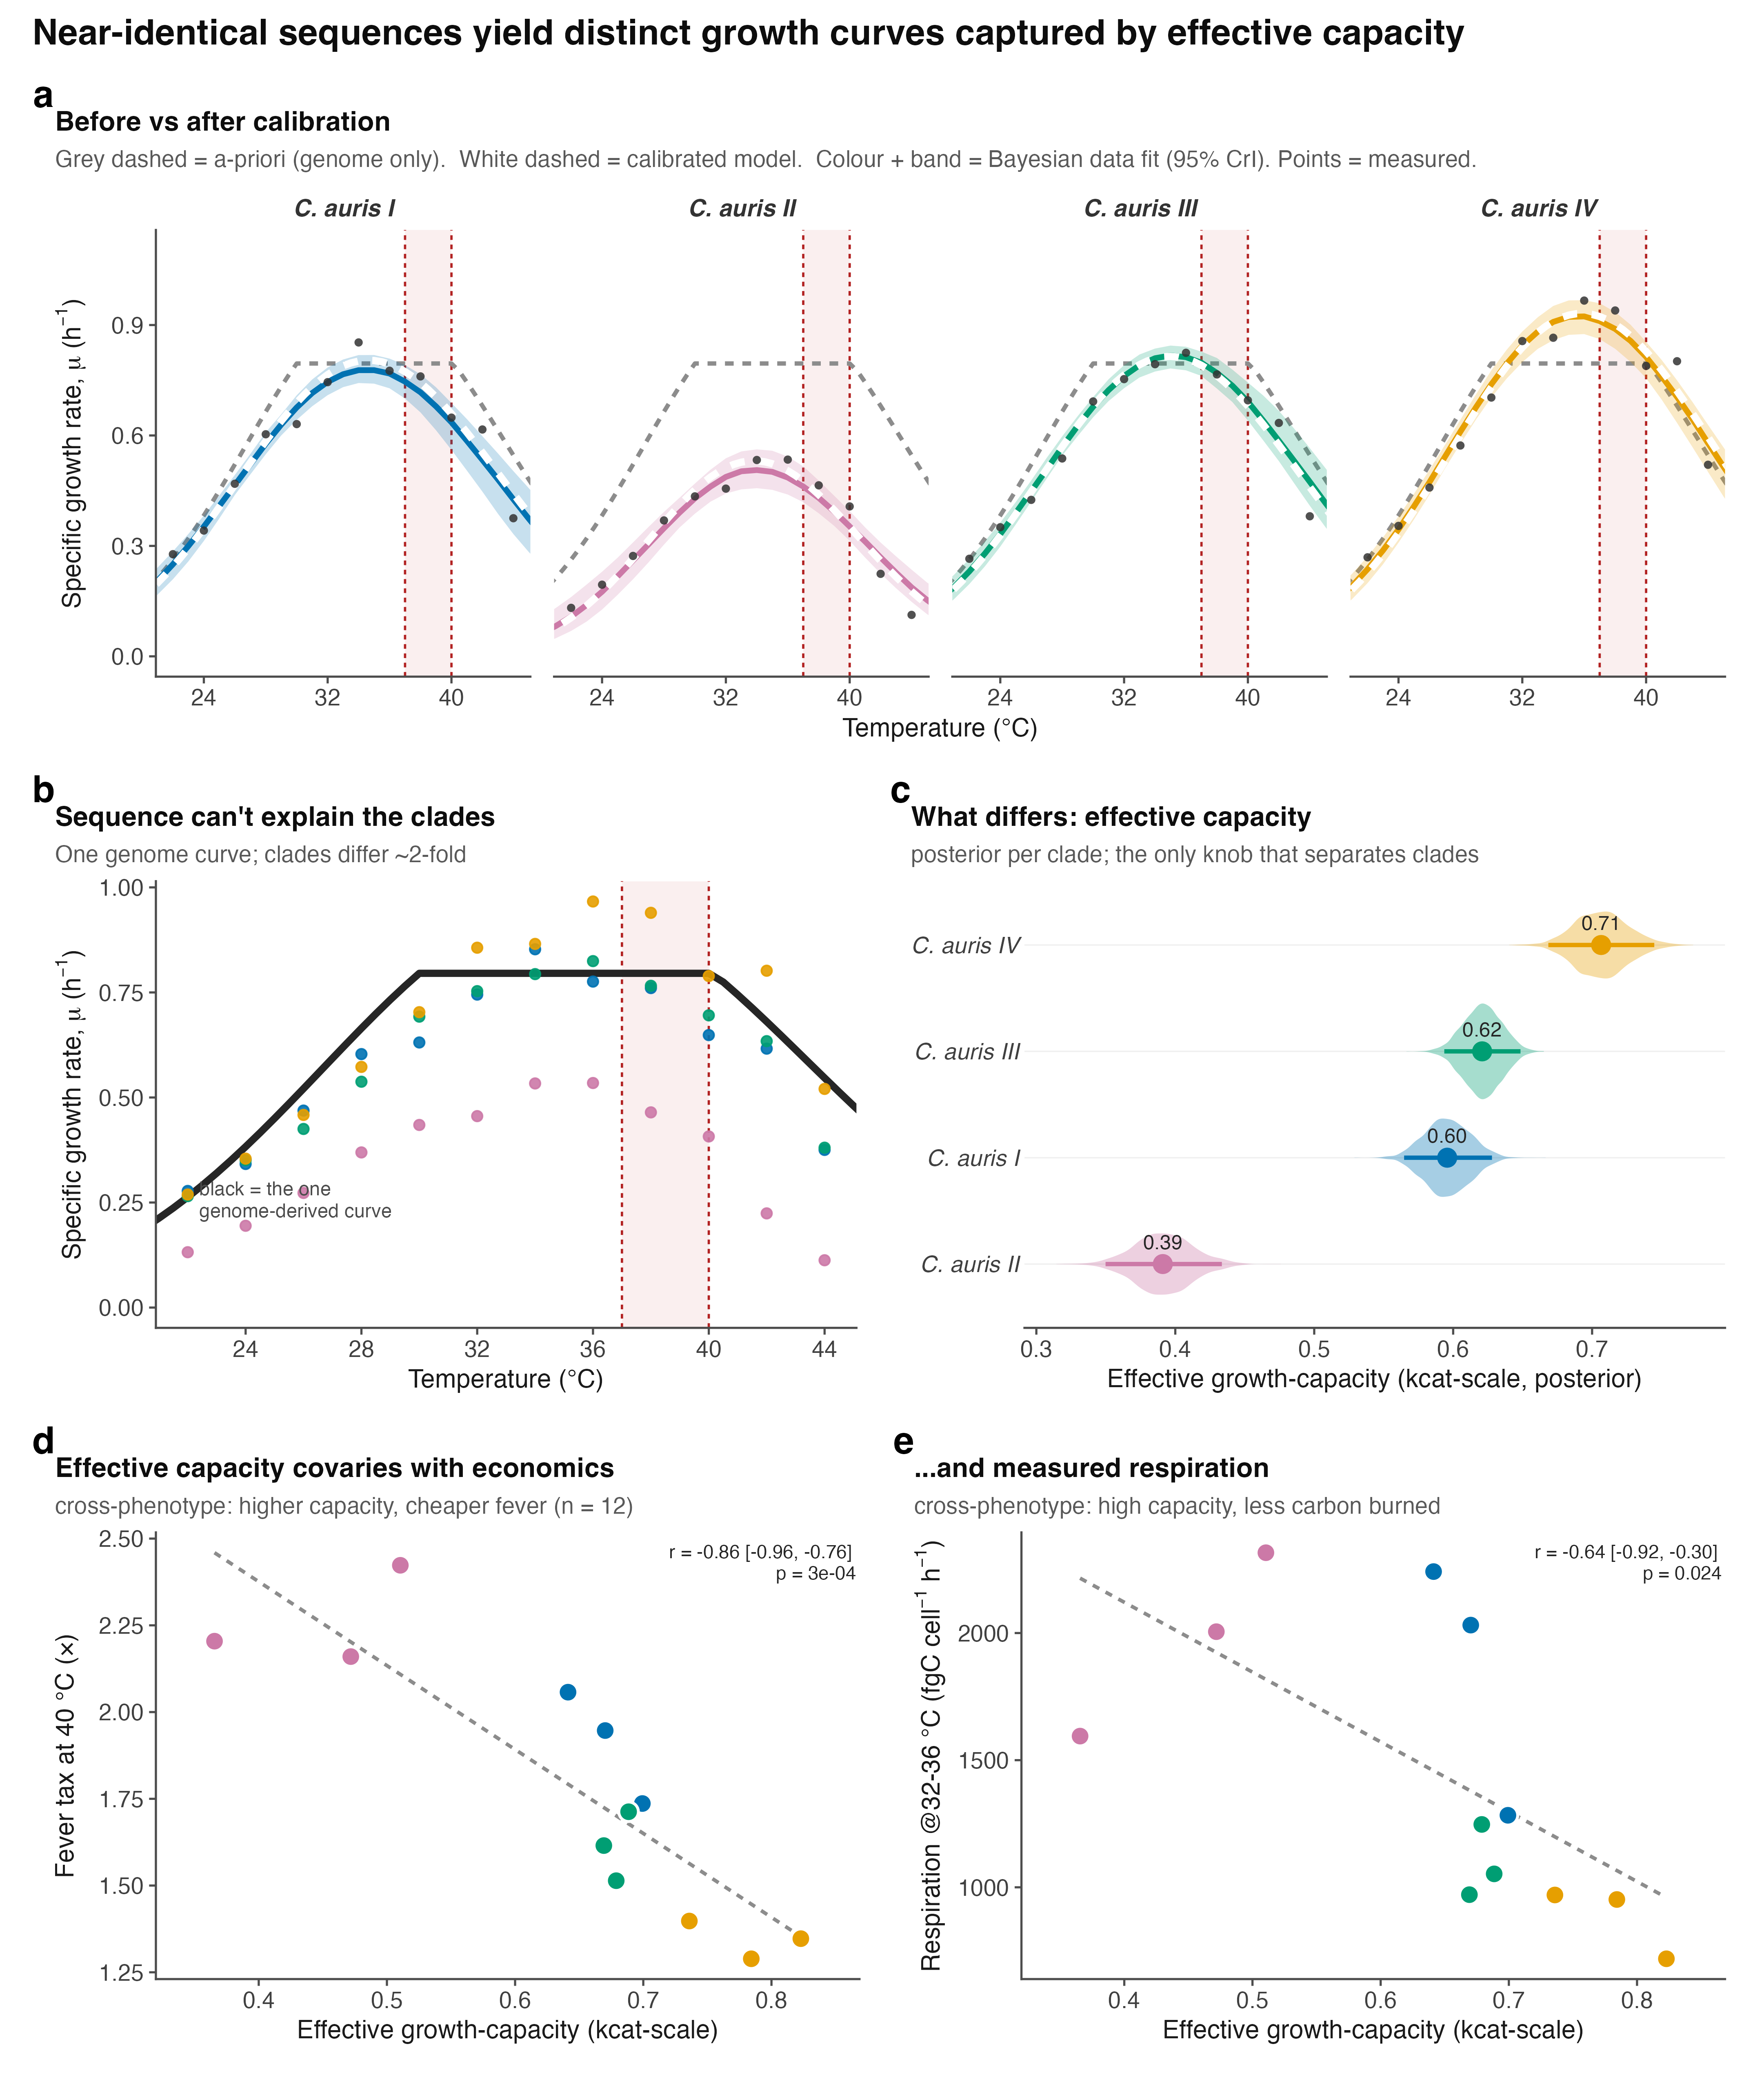
\includegraphics[width=6.39583in,height=7.51459in]{media/media/image4.png}

\textbf{Figure 4.} Clade differences are captured by an effective
growth-capacity axis despite near-identical sequence. (a) Per-clade
calibration of the sequence-grounded etc-GEM: grey dashed, genome-only
(a-priori) prediction; white dashed, calibrated model; colour and band,
Bayesian data fit (95\% CrI); points, measured. (b) The genome yields
one curve for all clades (black), yet the measured clades differ
\textasciitilde2-fold. (c) Posterior of the effective growth-capacity
parameter (kcat-scale) per clade; the only calibration parameter that
separates the clades. (d) Effective growth-capacity versus the measured
fever tax at 40 °C and (e) versus per-cell respiration at 32--36 °C
(points, twelve isolates coloured by clade). The scalar was fitted to
growth only; d--e are cross-phenotype associations, not independent
mechanistic validation, because the fever tax derives from measured
growth and respiration and the model's respiration at fixed growth is
not uniquely determined (see text). They replace the earlier
capacity-versus-growth panel, a self-consistency check (Supplementary
Fig. 2).

\textbf{Robustness and limitations}

Per-cell respiration and carbon-use efficiency depend on the starting
cell number N0, obtained by back-projecting the measured inoculum over
the pre-fit interval, N0 = N\_inoc·exp(r·Δt). The specific growth rate r
and its activation energy are recovered directly from the oxygen
dynamics and are independent of N0; only the per-cell respiratory flux,
CUE and quantities derived from them inherit its uncertainty, so we
assessed the two ways the back-projection can bias them. First, a
fit-window selection issue was corrected: for a small number of series
(chiefly at 26 °C) the selector had latched onto a short late-run
segment and returned implausible growth rates. These windows were
reviewed and corrected to span the full respiration phase, restoring the
expected unimodal growth curves and leaving every clade optimum in the
34--36 °C range.

Second, and more consequentially, the vials are inoculated near bench
temperature and take tens of minutes to reach setpoint, so the growth
accrued during the pre-fit interval is not governed by the stable r used
in the back-projection. Using the continuously logged internal vial
temperature together with each clade's own measured growth--temperature
curve, we recomputed the growth actually accrued during equilibration
and propagated the difference into N0. Growth per cell is unaffected by
construction. Per-cell respiration and CUE shift in a
temperature-structured way: negligibly across 22--36 °C, then
increasingly toward the extremes, with the sign set by the growth
optimum (below it, a cooler onset implies slower early growth and
slightly higher per-cell respiration; above it, the reverse). The median
shift on respiration reaches about +14\% near 30 °C and −27\% at 44 °C,
mirrored and buffered in CUE, while growth per cell is immune throughout
(Supplementary Fig. 3). Shown on the thermal curves themselves, widening
each posterior credible interval by this component leaves an outer
envelope that coincides with the credible interval through the mid-range
and separates only toward the extremes (Supplementary Figs. 4 and 5).

This equilibration correction is roughly an order of magnitude smaller
than the trends it could threaten: the CUE optimum still lies below 37
°C in every taxon, growth remains credibly more temperature-sensitive
than respiration, and respiration's monotonic rise is unchanged. We
therefore keep the per-cell point estimates unchanged but treat their
absolute values at the temperature extremes (≥40 °C) as approximate.

A stronger stress test is to remove the back-projection term entirely
(N0 = N\_inoc), the opposite bound to the equilibration correction. This
is not the physical null---the inoculum did grow before the fit window,
which is what the back-projection accounts for---so the true values lie
between it and the published table rather than at either end; but it
isolates every quantity that leans on the term. The primary conclusions
are unchanged or strengthened under it: r and its activation energy are
independent of N0 by construction, and the sub-37 °C CUE optimum in fact
sharpens. Two secondary results are sensitive and we report them
accordingly. First, the fine fever-cost ordering among the C.
\emph{auris} clades: Clade IV has the lowest respiration activation
energy with the term but not without it (its rank moves from first to
fourth of five), whereas the C. \emph{auris}-versus-\emph{C.
parapsilosis} contrast survives both bounds; we therefore state the
within-\emph{auris} ranking as conditional on the back-projection.
Second, the capacity-versus-respiration association of Fig. 4e, which
weakens to r ≈ −0.2 (not significant) under the same test and is read as
exploratory. The between-clade respiration activation energy under all
three treatments---with the term (published), equilibration-corrected,
and term-free---is compared directly in Supplementary Fig. 6.

Separately, the absolute carbon scale carries a systematic uncertainty
from the assumed respiratory quotient and per-cell carbon content;
varying these within literature ranges rescales CUE proportionally but
does not change its thermal shape, its sub-37 °C optimum, or any
among-taxon ranking. The primary conclusions in the preceding
sections---the sub-37 °C carbon-economy optimum, the growth-respiration
decoupling, and the C. \emph{auris}-versus-\emph{C. parapsilosis}
fever-cost contrast---are robust to all of these sources; the finer
within-\emph{auris} ordering and the Fig. 4e association are reported as
conditional on the inoculum back-projection.

Across the \emph{Candida} taxa tested, host and fever temperatures lie
above the optimum for carbon-use efficiency, because respiration
continues to rise after growth has peaked. The resulting fever cost is
smallest in the warmest-adapted \emph{C. auris} clade. A
sequence-grounded model reproduces the clade growth differences through
a single effective-capacity parameter that also covaries with
respiratory phenotype, but the molecular and bioenergetic basis of that
capacity remains unresolved.

\section{}\label{section}

\section{}\label{section-1}

\section{\texorpdfstring{\textbf{Supplementary
figures}}{Supplementary figures}}\label{supplementary-figures}

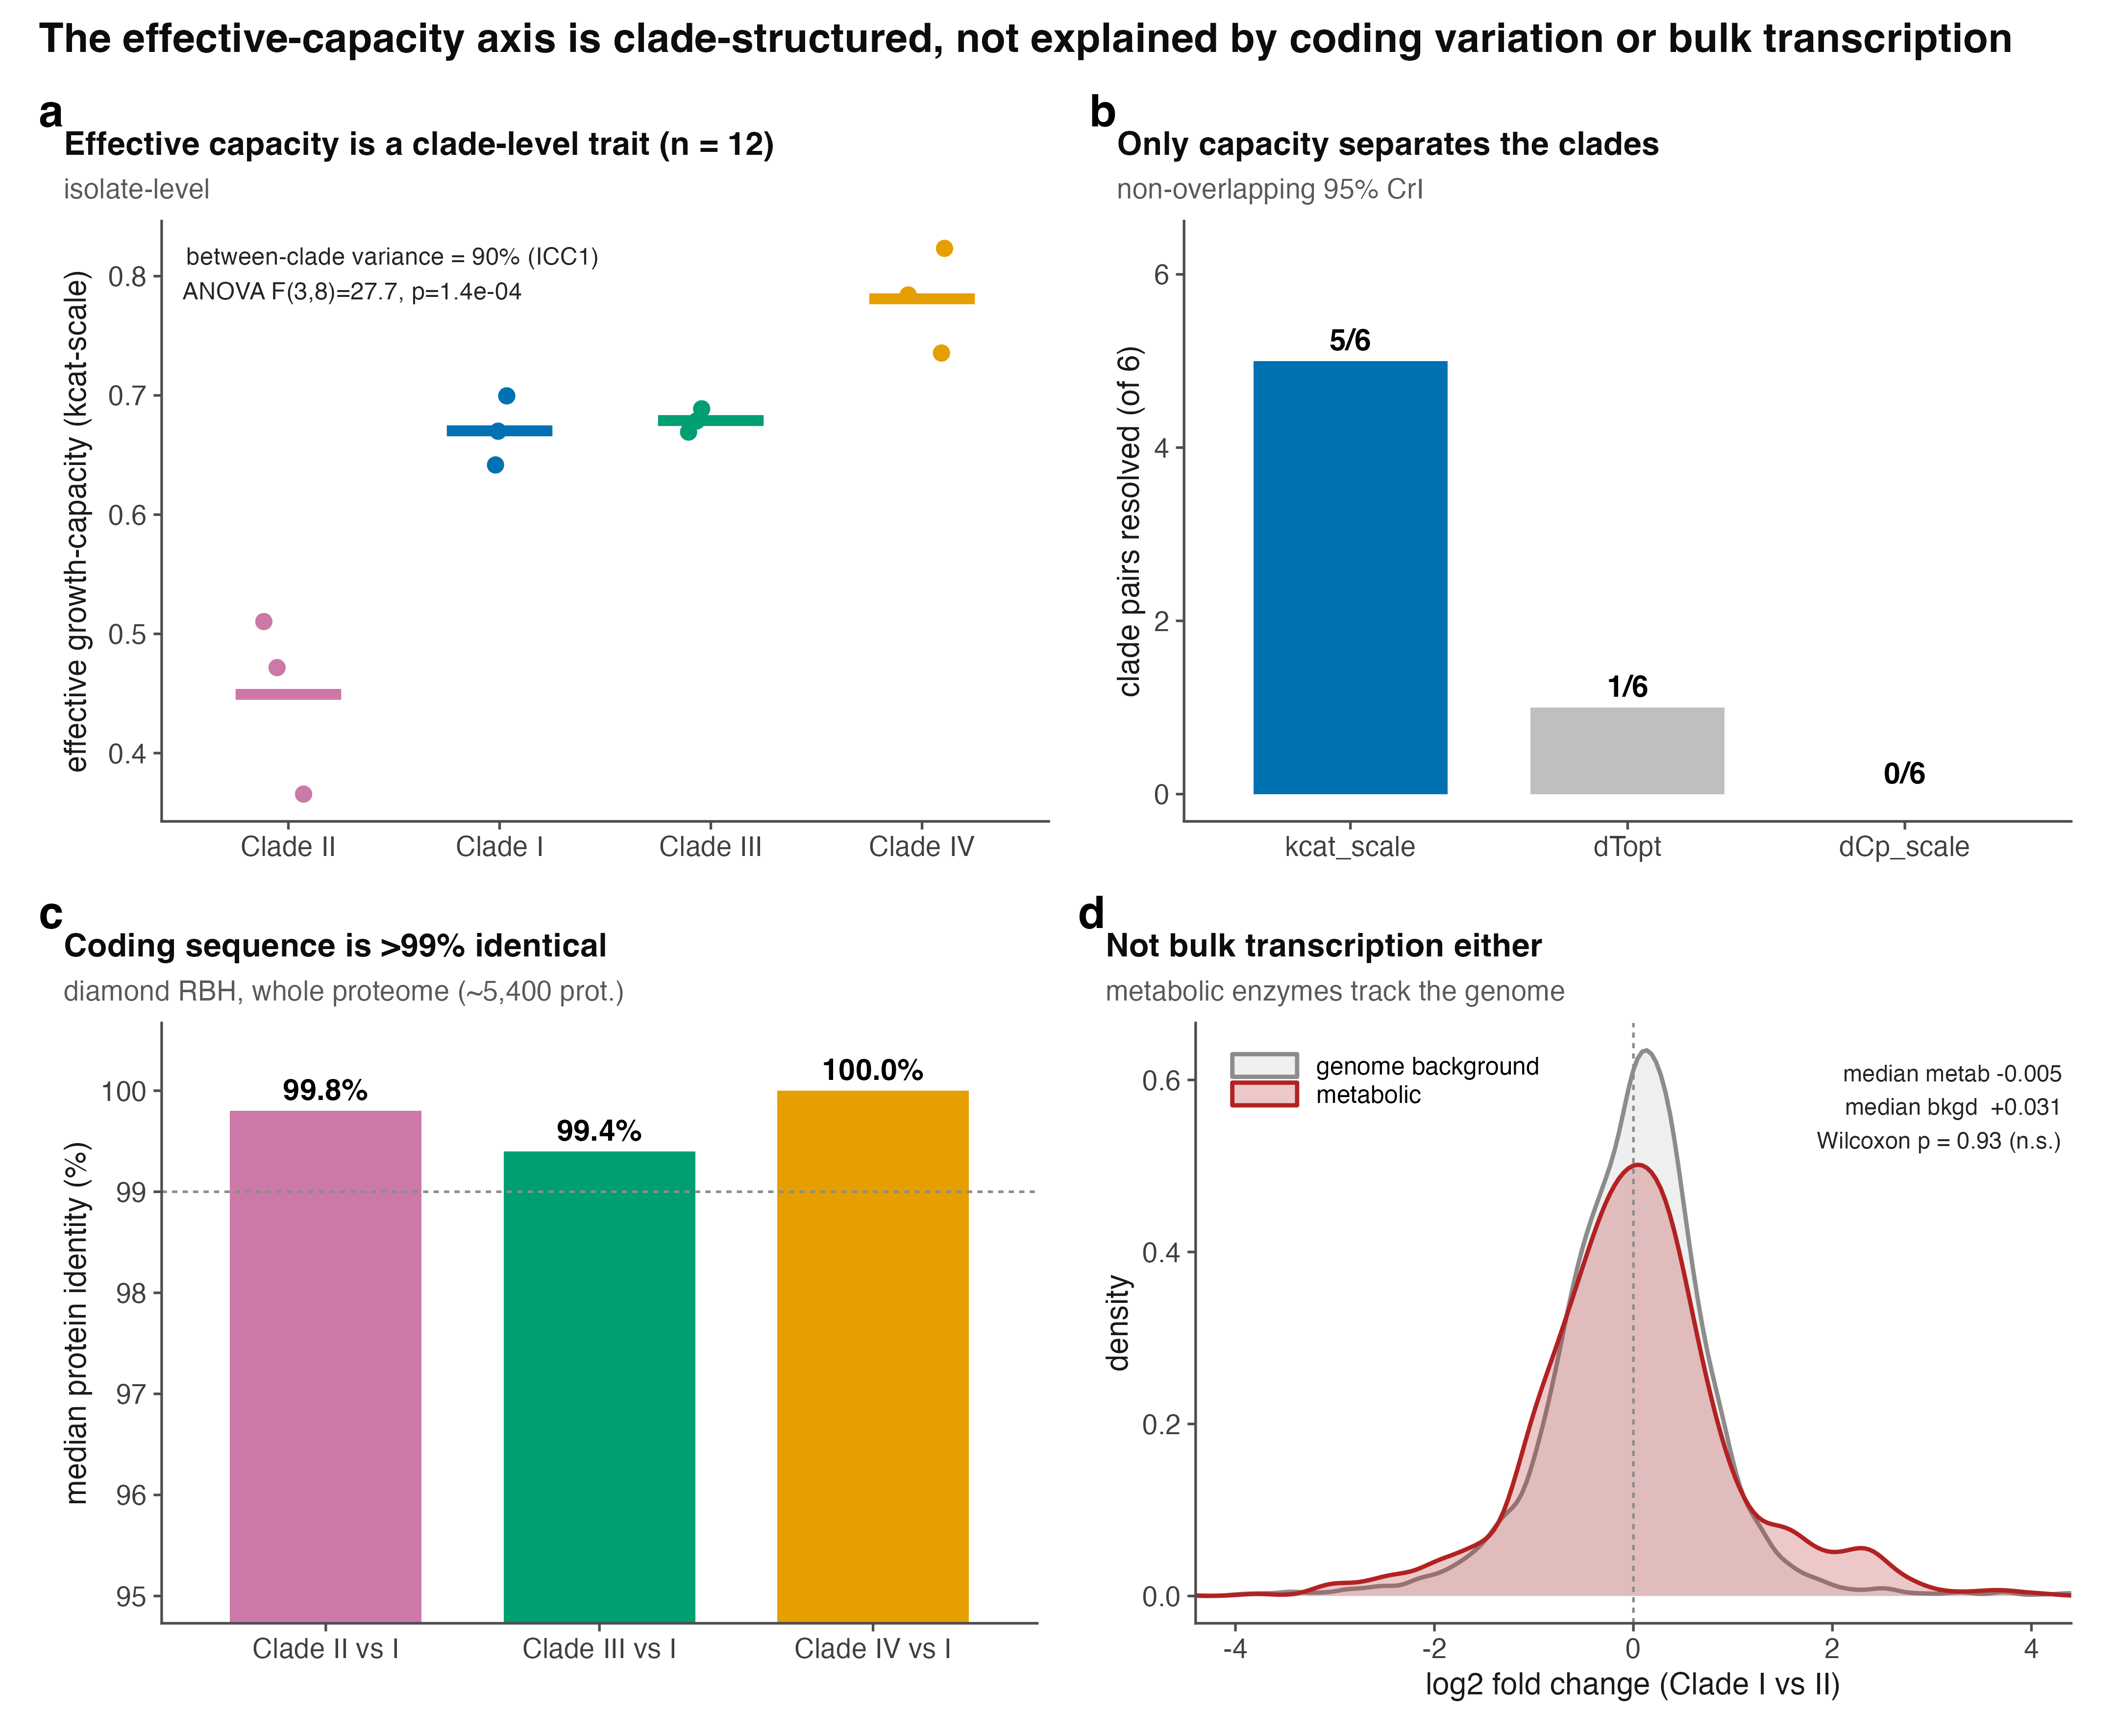
\includegraphics[width=6.39583in,height=5.24304in]{media/media/image5.png}

\textbf{Supplementary Figure 1.} The effective-capacity axis is
clade-structured and is not explained by coding variation or by
coordinated metabolic-transcript allocation in the available dataset.
(a) Capacity across the twelve isolates by clade (bars, clade means);
90\% of the variance lies between clades (ICC₁ = 0.90). (b) Number of
clade pairs resolved (non-overlapping 95\% CrI) by each calibration
parameter; only the effective growth-capacity parameter (kcat-scale)
separates the clades. (c) Median whole-proteome amino-acid identity of
each clade to Clade I (diamond reciprocal best-hit); coding sequence is
\textgreater99\% identical. (d) Distribution of Clade I-versus-II log₂
fold-change for the model's 928 metabolic-enzyme genes (red) against the
genome background (grey), from GEO GSE165762; the metabolic set is not
coordinately shifted (Wilcoxon P = 0.93).

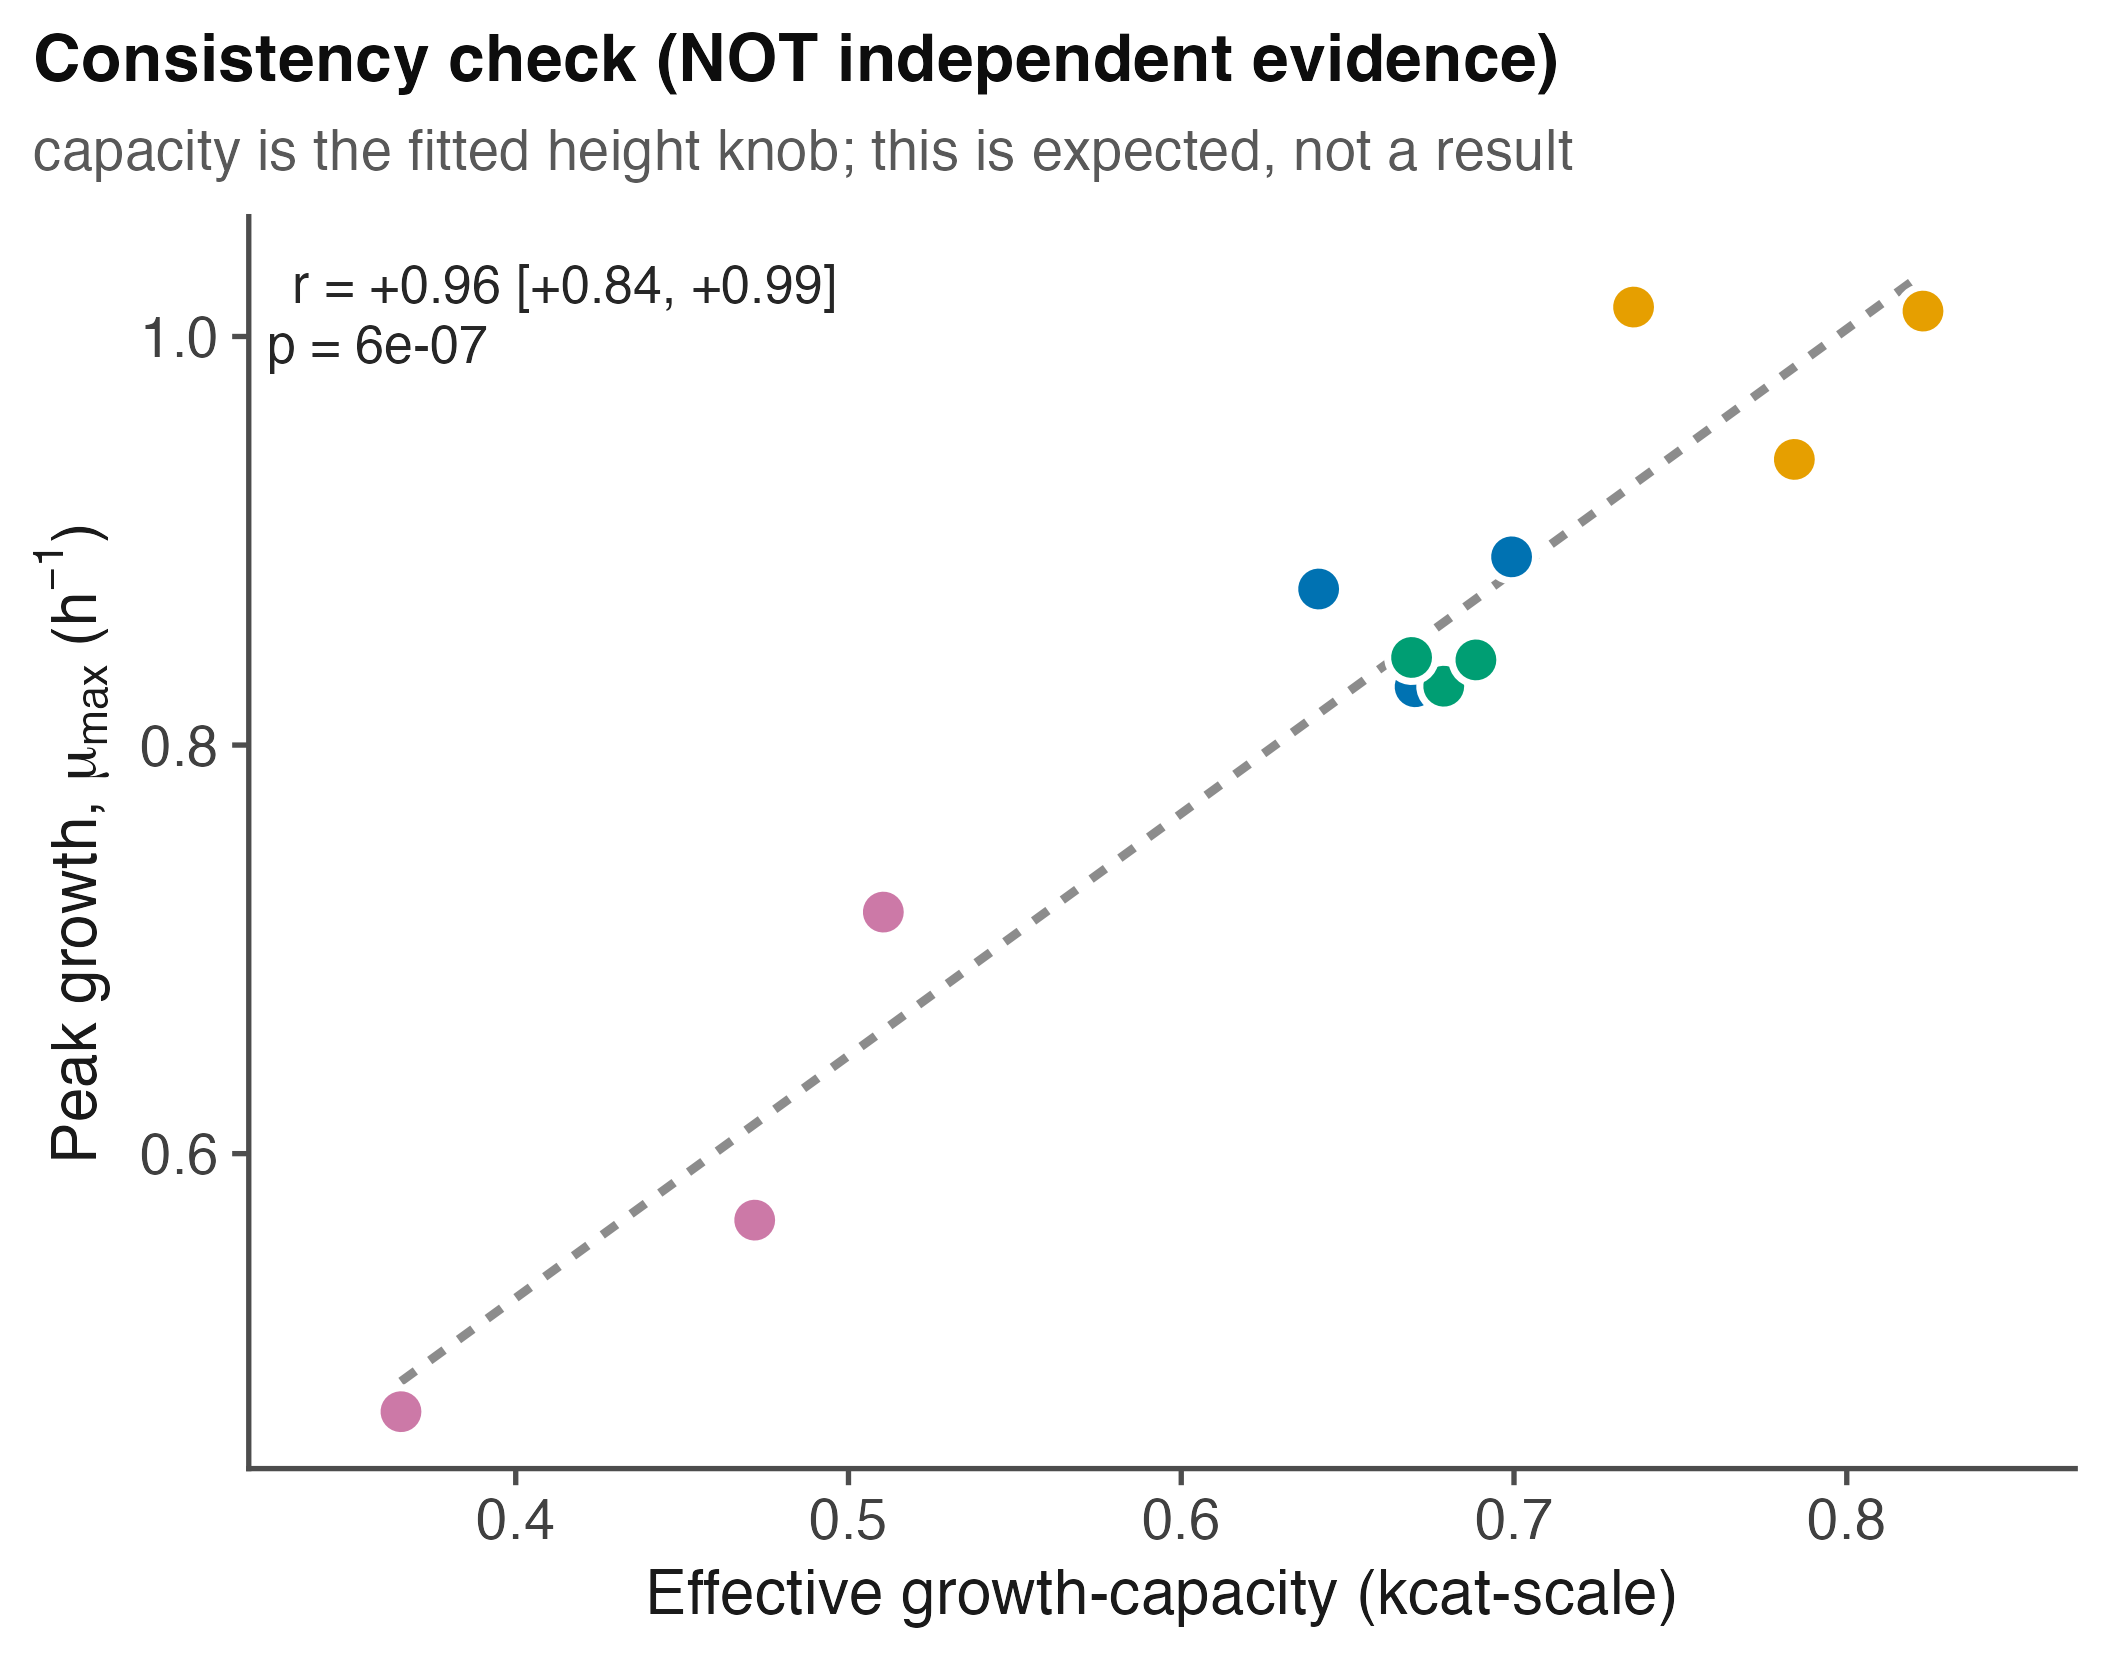
\includegraphics[width=6.39583in,height=4.97521in]{media/media/image6.png}

\textbf{Supplementary Figure 2.} Self-consistency check. Effective
growth-capacity (the fitted curve-height parameter) versus measured peak
growth across the twelve isolates (r = 0.96). Because capacity scales
curve height by construction, this relationship is expected and is shown
as a consistency check, not as independent evidence; the out-of-sample
tests are in Fig. 4d--e.

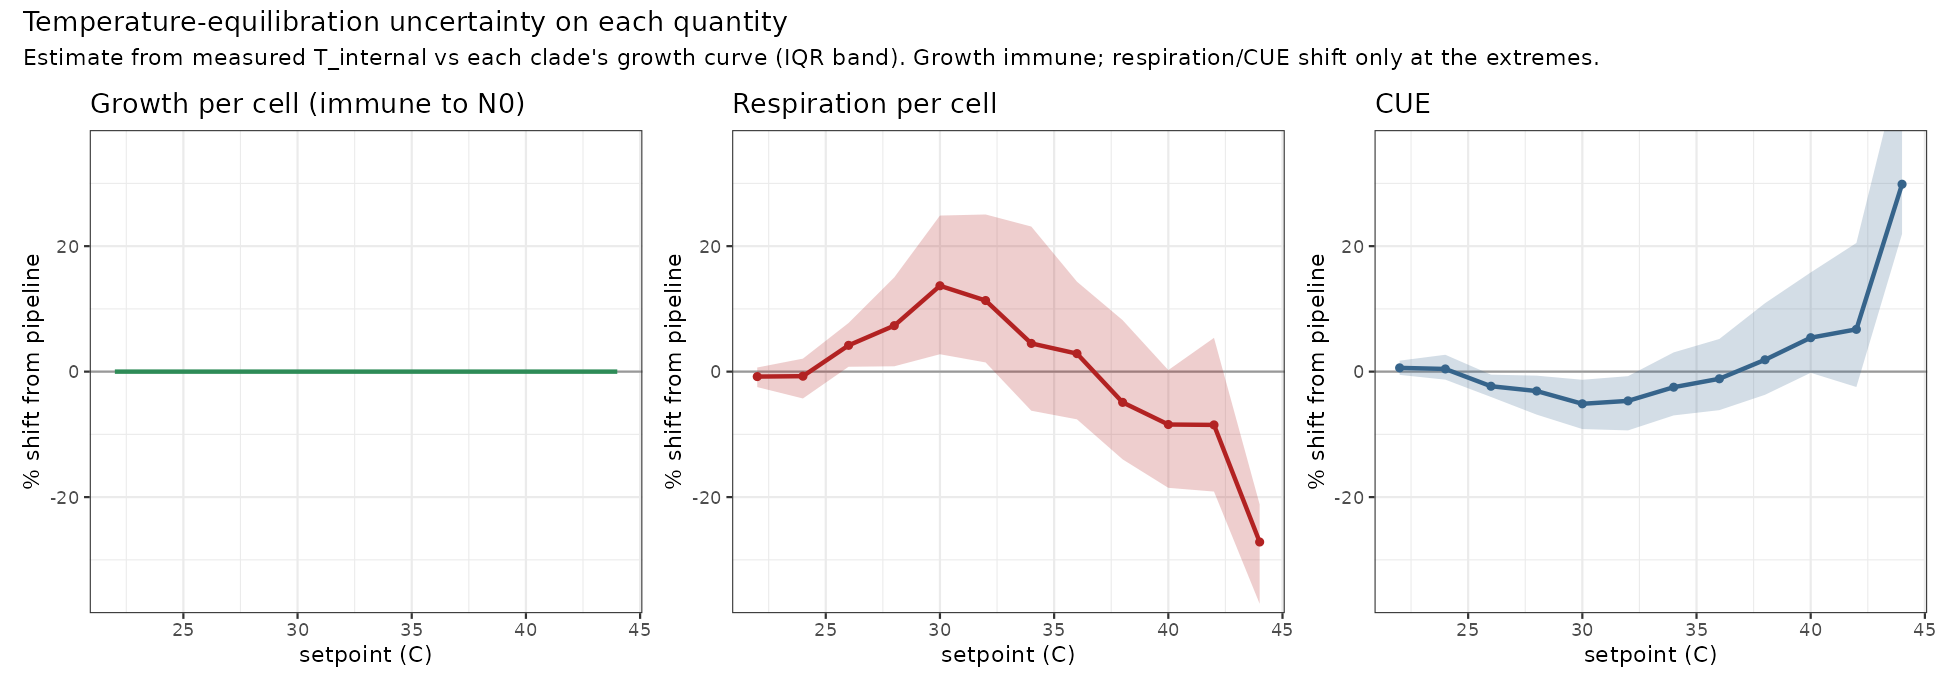
\includegraphics[width=6.6in,height=2.33538in]{media/media/image7.png}

\textbf{Supplementary Figure 3.} Sensitivity of each per-cell quantity
to temperature equilibration. Median percentage shift from the pipeline
value versus setpoint, estimated from the logged internal vial
temperature against each clade's growth curve (band, interquartile range
across vials). Growth per cell is immune because it does not use N0;
per-cell respiration shifts by a few percent through the mid-range and
up to about −27\% at 44 °C; CUE follows, buffered.

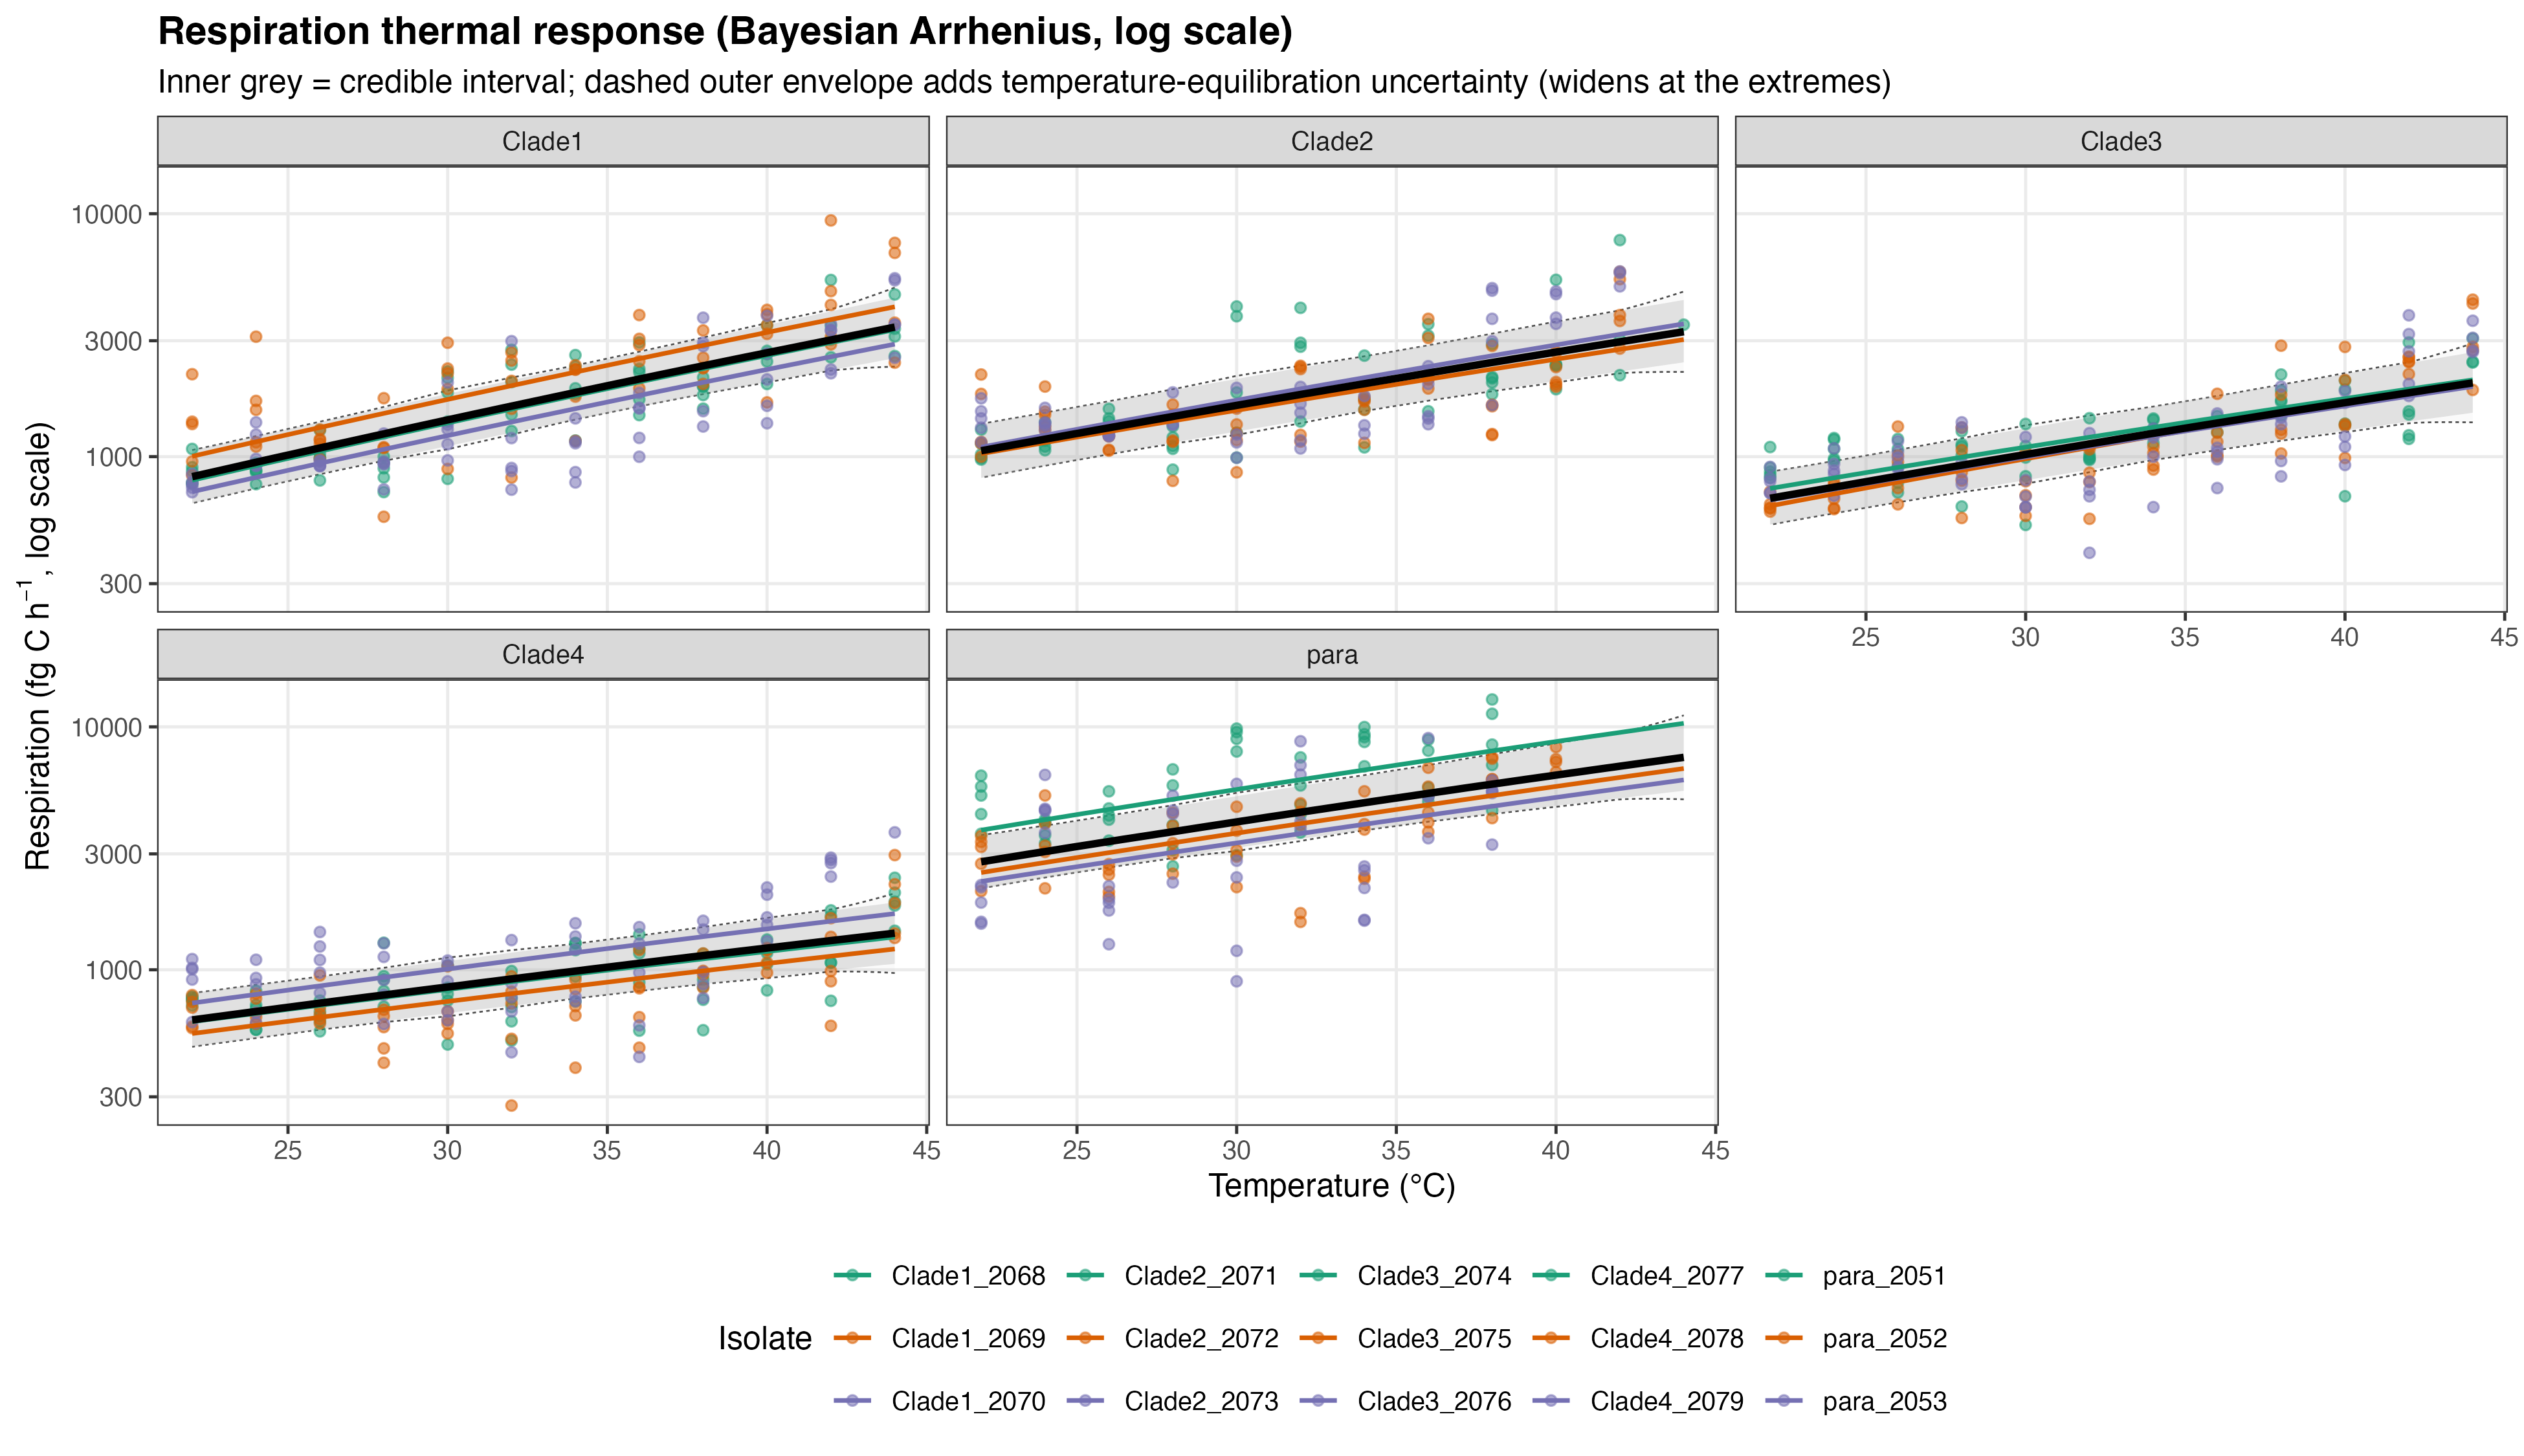
\includegraphics[width=6.6in,height=3.80769in]{media/media/image8.png}

\textbf{Supplementary Figure 4.} Per-cell respiration versus temperature
(Bayesian Arrhenius, log scale), per clade, with the
temperature-equilibration uncertainty overlaid. Solid band, 95\%
credible interval; dashed envelope, the same interval widened by the
equilibration component. The two coincide through the mid-range and
separate only toward the extremes; respiration's monotonic rise is
unaffected.

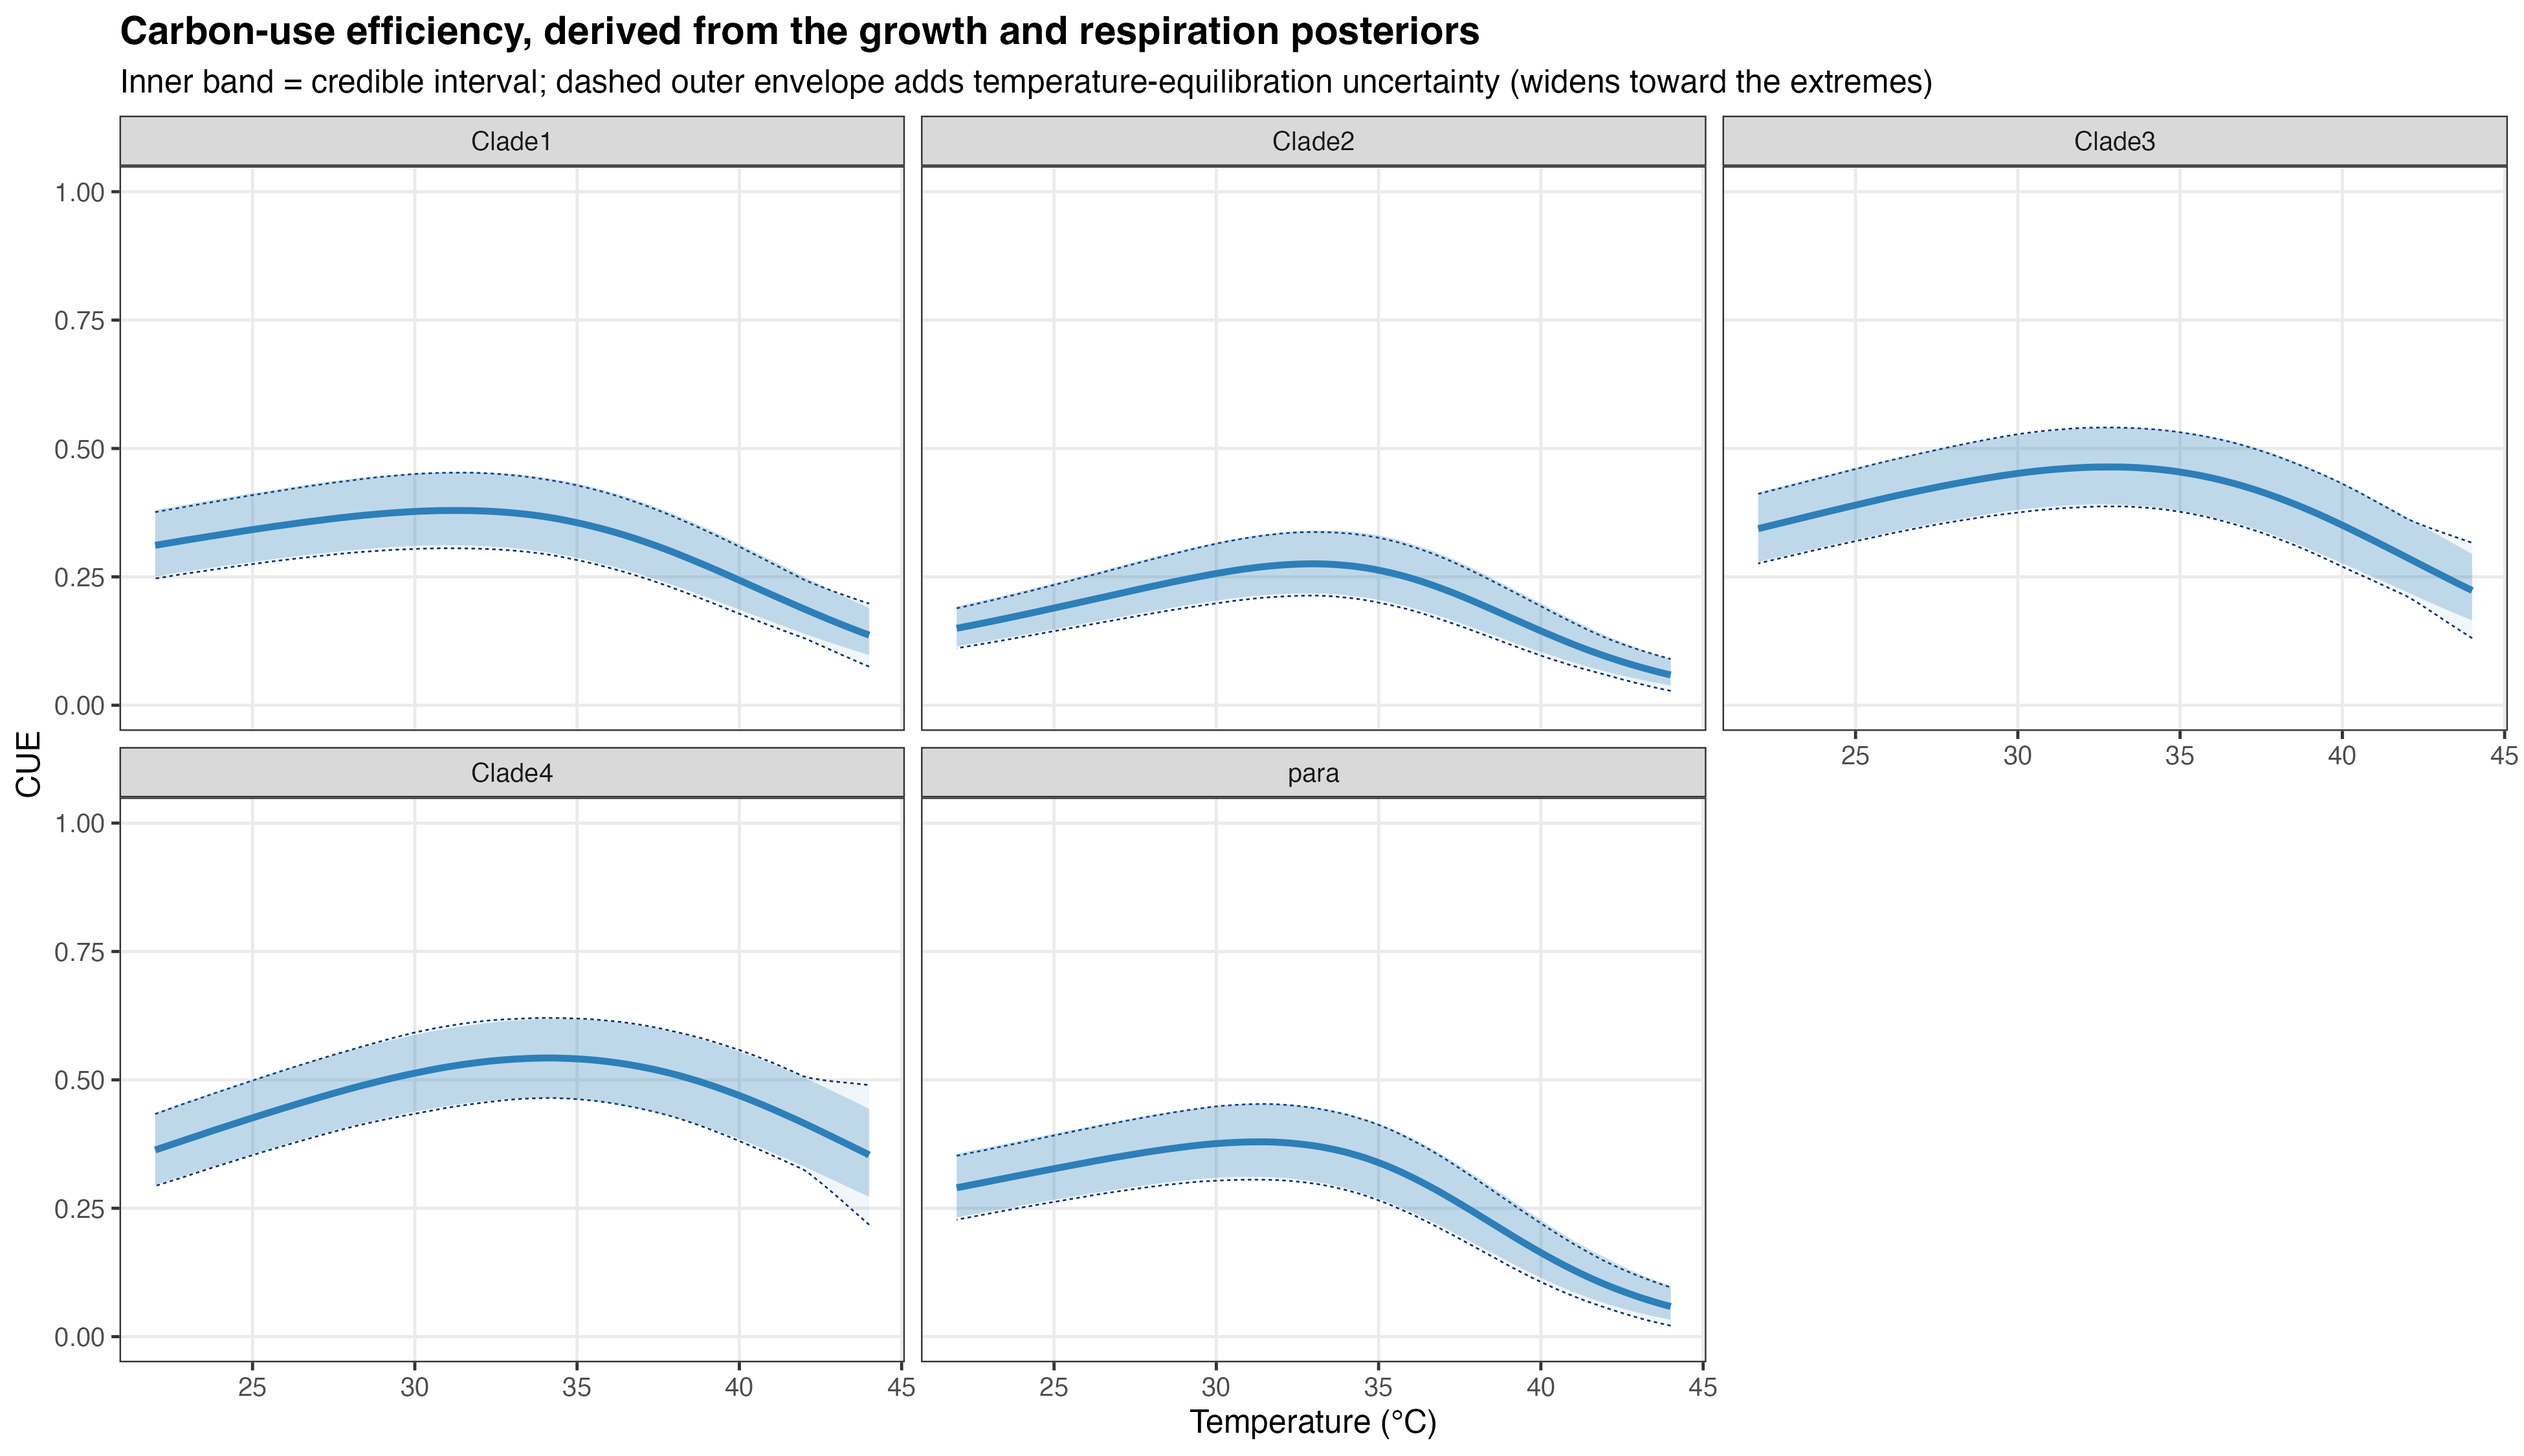
\includegraphics[width=6.6in,height=3.80769in]{media/media/image9.png}

\textbf{Supplementary Figure 5.} Carbon-use efficiency versus
temperature, per clade, with the temperature-equilibration uncertainty
overlaid. Solid band, 95\% credible interval; dashed envelope, widened
by the equilibration component. Even with the added uncertainty, CUE
peaks below body temperature and declines with further warming in every
clade.

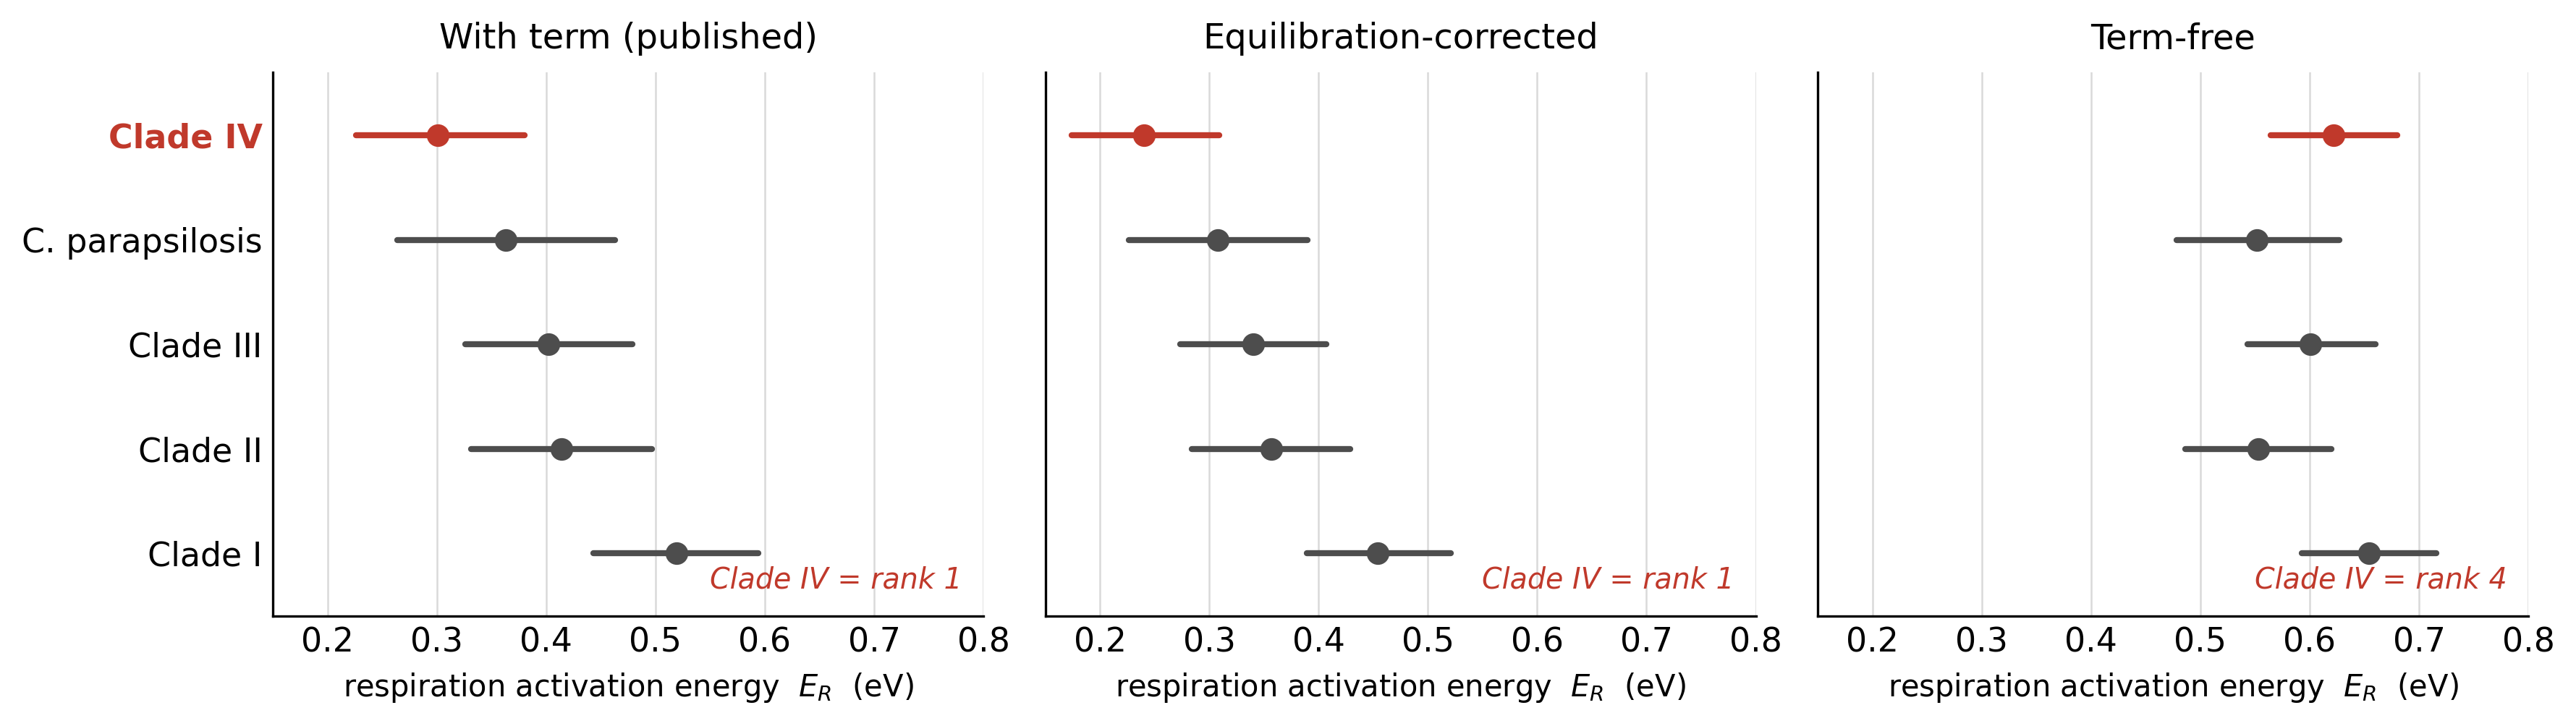
\includegraphics[width=6.6in,height=3in]{media/media/image10.png}

\textbf{Supplementary Figure 6.} The between-clade respiration
activation energy under three treatments of the inoculum
back-projection. Each panel shows the hierarchical Bayesian Arrhenius
activation energy E\textsubscript{R} per clade (posterior median; bars,
95\% credible interval), refitting the same model under: (left) the
published back-projection, N0 = N\_inoc·exp(r·Δt); (centre) the
equilibration-corrected N0, recomputed from the logged internal vial
temperature over the onset window; and (right) the term removed
entirely, N0 = N\_inoc. The C. \emph{auris}-versus-\emph{C.
parapsilosis} separation is preserved across all three, but the finer
ordering within C. \emph{auris} is not: Clade IV holds the lowest
activation energy under the published and equilibration-corrected
treatments and moves to fourth of five when the term is removed. The
term-free case is not the physical null (the inoculum grows before the
fit window), so it bounds the correction from the opposite side rather
than representing the correct value; it is shown to make the dependence
explicit. Generated by \texttt{scripts/16b\_n0\_treatment\_panel.R}.

\section{}\label{section-2}

\section{\texorpdfstring{\textbf{Reference}}{Reference}}\label{reference}

Cakin I, Millington R, Pawar S, Buckling A, Smirnoff N, Padfield D,
Duffy J, Yvon-Durocher G. \emph{A novel method to simultaneously
estimate bacterial respiration and growth from oxygen dynamics.} ISME
Communications 2026;6(1):ycag024. https://doi.org/10.1093/ismeco/ycag024




\end{document}
